\documentclass[aspectratio=169]{beamer}
% ============================================================================
% HEC Montréal MBA -- ECON50803: Macroeconomic Environment
% Shared Beamer Preamble
% ============================================================================

% --- Theme and base settings ------------------------------------------------
\usetheme{default}
\setbeamersize{text margin left=1.2cm, text margin right=1.2cm}

% --- Fonts ------------------------------------------------------------------
% Sans-serif throughout for a business look (comment out FiraSans if unavailable)
\usepackage[sfdefault,light]{FiraSans}
\usepackage{FiraMono}
\usepackage[T1]{fontenc}
\usepackage[utf8]{inputenc}
\setbeamerfont{title}{series=\bfseries, size=\Large}
\setbeamerfont{frametitle}{series=\bfseries, size=\large}
\setbeamerfont{framesubtitle}{series=\mdseries, size=\normalsize}

% --- Colors -----------------------------------------------------------------
\definecolor{HECnavy}{HTML}{002855}
\definecolor{HECgreen}{HTML}{26d07c}
\definecolor{HECcoral}{HTML}{ff585d}
\definecolor{HECtext}{HTML}{2D3748}
\definecolor{HECgray}{HTML}{94A3B8}
\definecolor{HEClightgray}{HTML}{F1F5F9}
\definecolor{HEClightblue}{HTML}{E8EDF3}

% Beamer color assignments
\setbeamercolor{normal text}{fg=HECtext}
\setbeamercolor{title}{fg=HECnavy}
\setbeamercolor{frametitle}{fg=HECnavy}
\setbeamercolor{structure}{fg=HECnavy}
\setbeamercolor{background canvas}{bg=white}
\setbeamercolor{alerted text}{fg=HECcoral}
\setbeamercolor{example text}{fg=HECgreen}
\hypersetup{colorlinks, linkcolor=HECnavy, urlcolor=HECnavy, citecolor=HECtext}

% --- Navigation and chrome --------------------------------------------------
\setbeamertemplate{navigation symbols}{}

% Frame title: bold text with a thin accent line
\setbeamertemplate{frametitle}{%
   \vspace{0.25cm}%
   {\usebeamerfont{frametitle}\usebeamercolor[fg]{frametitle}\insertframetitle}%
   \ifx\insertframesubtitle\empty\else%
      \\[2pt]{\usebeamerfont{framesubtitle}\textcolor{HECgray}{\insertframesubtitle}}%
   \fi%
   \\[-4pt]\textcolor{HECgreen}{\rule{2.5cm}{1.5pt}}%
   \\[-2pt]%
}

% Footer: course name left, slide number right, thin rule above
\setbeamertemplate{footline}{%
   \vspace{-0.1cm}%
   \hbox to \paperwidth{%
      \hspace{1.2cm}%
      \textcolor{HEClightgray}{\rule{0.84\paperwidth}{0.4pt}}%
      \hspace{1.2cm}%
   }%
   \vspace{0.05cm}%
   \hbox to \paperwidth{%
      \hspace{1.2cm}%
      {\scriptsize\textcolor{HECgray}{ECON 50803\enspace\textbar\enspace Environnement macroéconomique}}%
      \hfill%
      {\scriptsize\textcolor{HECgray}{\insertframenumber}}%
      \hspace{1.2cm}%
   }%
   \vspace{0.15cm}%
}

% --- Itemize/enumerate styling ----------------------------------------------
\setbeamertemplate{itemize item}{\textcolor{HECnavy}{$\bullet$}}
\setbeamertemplate{itemize subitem}{\textcolor{HECgray}{$\bullet$}}
\setbeamertemplate{itemize subsubitem}{\textcolor{HECgray}{\scalebox{0.6}{$\blacktriangleright$}}}
\setbeamertemplate{enumerate item}{\textcolor{HECnavy}{\bfseries\insertenumlabel.}}
\setbeamertemplate{enumerate subitem}{\textcolor{HECgray}{\insertsubenumlabel.}}

% --- Packages ---------------------------------------------------------------
\usepackage{
   tikz, caption, subcaption, ragged2e, amsmath, bm,
   makecell, threeparttable, booktabs, mathtools,
   multirow, calc, hyperref, tabularx, colortbl,
   transparent, tcolorbox, xcolor, graphicx
}
\usepackage[round]{natbib}
\usetikzlibrary{decorations.pathreplacing, decorations.markings, calc, arrows.meta, positioning}
\usepackage[absolute,overlay]{textpos}
\captionsetup[figure]{labelformat=empty, font=small, textfont=it}
\captionsetup[table]{labelformat=empty, font=small}
\setlength{\belowcaptionskip}{0cm}
\apptocmd{\frame}{}{\justifying}

% --- Paths ------------------------------------------------------------------
\graphicspath{{../Figures/}}
\newcommand*\includetables[1]{\input{../Tables/#1.tex}}

% --- Mathematical commands --------------------------------------------------
\DeclareMathOperator*{\argmax}{arg\,max}
\newcommand{\partialof}[2]{\frac{\partial #1}{\partial #2}}
\newcommand{\totalof}[2]{\frac{\text{d}#1}{\text{d}#2}}
\newcommand{\pctchg}[1]{\%\Delta #1}
\newcommand{\smallquad}{\hspace{0.5em}}

% --- Resize equation command ------------------------------------------------
\newcommand{\resizeeq}[2]{\resizebox{#2\hsize}{!}{$#1$}}

% ============================================================================
% CUSTOM SLIDE TYPES
% ============================================================================

% --- Title slide (call with \titleframe) ------------------------------------
\newcommand{\titleframe}{%
   {\setbeamertemplate{footline}{}%
   \begin{frame}[plain]
      \begin{tikzpicture}[remember picture, overlay]
         % Navy accent bar on the left
         \fill[HECnavy] (current page.north west) rectangle
            ([xshift=0.6cm]current page.south west);
         % Green accent line
         \fill[HECgreen] ([xshift=0.6cm]current page.north west) rectangle
            ([xshift=0.65cm]current page.south west);
      \end{tikzpicture}
      \vspace{1cm}
      \hspace{0.6cm}%
      \begin{minipage}{0.85\textwidth}
         {\usebeamerfont{title}\usebeamercolor[fg]{title}\inserttitle}
         \\[12pt]
         \textcolor{HECgreen}{\rule{3cm}{2pt}}
         \\[12pt]
         {\large\textcolor{HECgray}{\insertauthor}}
         \\[6pt]
         {\normalsize\textcolor{HECgray}{\insertdate}}
      \end{minipage}
      \vfill
      \hspace{0.6cm}%
      {\footnotesize\textcolor{HECgray}{HEC Montréal \enspace\textbar\enspace MBA}}
      \vspace{0.5cm}
   \end{frame}}%
}

% --- Section divider slide --------------------------------------------------
\newcommand{\sectionframe}[1]{%
   {\setbeamertemplate{footline}{}%
   \begin{frame}[plain]
      \begin{tikzpicture}[remember picture, overlay]
         \fill[HECnavy] ([shift={(-1pt,1pt)}]current page.north west) rectangle
            ([shift={(1pt,-1pt)}]current page.south east);
         \node[anchor=center] at (current page.center) {%
            \begin{minipage}{0.8\paperwidth}
               \centering
               {\LARGE\bfseries\textcolor{white}{#1}}
               \\[12pt]
               \textcolor{HECgreen}{\rule{3cm}{2pt}}
            \end{minipage}
         };
      \end{tikzpicture}
   \end{frame}}%
}

% ============================================================================
% CUSTOM BOX ENVIRONMENTS
% ============================================================================

% Key Insight (green accent)
\newtcolorbox{keyinsight}[1][Point clé]{%
   colback=HECgreen!5,
   colframe=HECgreen,
   boxrule=0pt,
   leftrule=3pt,
   arc=8pt,
   title={\textcolor{HECgreen}{\bfseries #1}},
   coltitle=HECgreen,
   fonttitle=\bfseries,
   attach title to upper={\\[4pt]},
   left=10pt, right=10pt, top=6pt, bottom=6pt
}

% Business Implication (navy accent)
\newtcolorbox{bizimplication}[1][Implication d'affaires]{%
   colback=HECnavy!5,
   colframe=HECnavy,
   boxrule=0pt,
   leftrule=3pt,
   arc=8pt,
   title={\textcolor{HECnavy}{\bfseries #1}},
   coltitle=HECnavy,
   fonttitle=\bfseries,
   attach title to upper={\\[4pt]},
   left=10pt, right=10pt, top=6pt, bottom=6pt
}

% Warning / Important (coral accent)
\newtcolorbox{warning}[1][Important]{%
   colback=HECcoral!5,
   colframe=HECcoral,
   boxrule=0pt,
   leftrule=3pt,
   arc=8pt,
   title={\textcolor{HECcoral}{\bfseries #1}},
   coltitle=HECcoral,
   fonttitle=\bfseries,
   attach title to upper={\\[4pt]},
   left=10pt, right=10pt, top=6pt, bottom=6pt
}

% Definition (gray background)
\newtcolorbox{defbox}[1][Définition]{%
   colback=HEClightgray,
   colframe=HEClightgray,
   boxrule=0pt,
   leftrule=3pt,
   arc=8pt,
   left=10pt, right=10pt, top=6pt, bottom=6pt,
   title={\textcolor{HECnavy}{\bfseries #1}},
   coltitle=HECnavy,
   fonttitle=\bfseries,
   attach title to upper={\\[4pt]}
}

% In-Class Exercise (coral accent)
\newtcolorbox{exercise}[1][Exercice]{%
   colback=HECcoral!5,
   colframe=HECcoral,
   boxrule=0pt,
   leftrule=3pt,
   arc=8pt,
   title={\textcolor{HECcoral}{\bfseries #1}},
   coltitle=HECcoral,
   fonttitle=\bfseries,
   attach title to upper={\\[4pt]},
   left=10pt, right=10pt, top=6pt, bottom=6pt
}

% ============================================================================
% NEWSPAPER HEADLINES SLIDE TEMPLATE
% ============================================================================
% Usage: inside a frame, open a tikzpicture[remember picture, overlay], then:
%   \setcounter{newshl}{0}
%   \newsheadline{Newspaper Name}{``Headline text''}   % up to 6 entries
%   \headlinesoverlay{Large overlay text}               % optional 2nd slide
%
% Headlines are auto-positioned in a 2×3 staggered grid (left/right alternating).
%
% Logo support: place PNG files in Figures/logos/ (e.g., ft.png, economist.png).
% Use the optional argument to specify the logo file (without extension):
%   \newsheadline[ft]{Financial Times}{Headline text}   % logo + bold headline
%   \newsheadline{The Economist}{``Headline text''}      % text-only fallback

\newcounter{newshl}

\newcommand{\newsheadline}[3][]{%
   % #1 = optional logo file key (e.g., ft → logos/ft.png)
   % #2 = newspaper name (text fallback when no logo)
   % #3 = headline text
   \stepcounter{newshl}%
   \pgfmathsetmacro{\hlrow}{int((\thenewshl-1)/2)}%
   \pgfmathsetmacro{\hlcol}{int(mod(\thenewshl-1,2))}%
   \pgfmathsetmacro{\hlx}{0.8 + \hlcol * 7.8}%
   \pgfmathsetmacro{\hly}{-1.5 - \hlrow * 2.0}%
   \node[anchor=north west]
      at ([shift={(\hlx cm,\hly cm)}]current page.north west) {%
      \ifx\\#1\\%
         \begin{minipage}[t]{5.8cm}%
            \textbf{\textcolor{HECgray}{\footnotesize\MakeUppercase{#2}}}%
            \\[-1pt]%
            {\small\itshape #3}%
         \end{minipage}%
      \else%
         \begin{minipage}[c]{1.2cm}%
            \includegraphics[height=1.2cm]{logos/#1}%
         \end{minipage}%
         \hspace{6pt}%
         \begin{minipage}[c][1.2cm][c]{4.3cm}%
            \raggedright{\small\textcolor{HECtext!75}{#3}}%
         \end{minipage}%
      \fi%
   };%
}

\newcommand{\headlinesoverlay}[1]{%
   \only<2>{%
      \fill[white, opacity=0.85]
         (current page.south west) rectangle (current page.north east);%
      \node[anchor=center] at ([yshift=-0.5cm]current page.center) {%
         {\fontsize{36}{44}\selectfont\bfseries\textcolor{HECnavy}{#1}}%
      };%
   }%
}

% ============================================================================
% NAVIGATION BUTTONS (optional, for bottom-of-slide section nav)
% ============================================================================

\newlength{\buttonwidth}
\newlength{\currentxpos}
\setlength{\currentxpos}{1.2cm}
\newlength{\buttonsep}
\setlength{\buttonsep}{0.05cm}

\newcommand{\mybutton}[2]{%
   \settowidth{\buttonwidth}{#1}%
   \begin{textblock*}{\buttonwidth + 2ex}(\currentxpos, \paperheight - 2.5em)
      \hyperlink{#2}{\beamerbutton{#1}}
   \end{textblock*}%
   \addtolength{\currentxpos}{\buttonwidth + \buttonsep}%
}

% ============================================================================
% BACKUP SLIDES SUPPORT
% ============================================================================

\newcommand{\backupbegin}{%
   \newcounter{finalframe}%
   \setcounter{finalframe}{\value{framenumber}}%
}
\newcommand{\backupend}{%
   \setcounter{framenumber}{\value{finalframe}}%
}


\title{Commerce international et économie ouverte}
\author{Jean-Félix Brouillette}
\date{Séance 6}

\begin{document}

% ============================================================================
\titleframe
% ============================================================================

% --- Opening hook: newspaper headlines ---
{
\setbeamertemplate{footline}{}
\begin{frame}{Le commerce mondial en question}
   \begin{tikzpicture}[remember picture, overlay]
      \setcounter{newshl}{0}
      \newsheadline[bloomberg]{Bloomberg}{\guillemotleft~On Trade and Tariffs, the World Is Moving on From the US~\guillemotright}
      \newsheadline[washpost]{The Washington Post}{\guillemotleft~Trump remakes U.S.\ trade strategy, with highest tariffs since 1930s~\guillemotright}
      \newsheadline[globeandmail]{The Globe and Mail}{\guillemotleft~U.S.\ trade policy toward Canada is far more restrictive than tariff rates suggest~\guillemotright}
      \newsheadline[ledevoir]{Le Devoir}{\guillemotleft~La guerre commerciale mondiale de Donald Trump n'est pas terminée~\guillemotright}
      \newsheadline[lapresse]{La Presse}{\guillemotleft~Un retour au libre-échange complet est peu probable, selon LeBlanc~\guillemotright}
      \newsheadline[radiocanada]{Radio-Canada}{\guillemotleft~Trump impose de nouveaux droits de douane à des dizaines de pays~\guillemotright}
   \end{tikzpicture}
\end{frame}
}

% ============================================================================
% PLAN
% ============================================================================

\begin{frame}{Plan}
   \begin{enumerate}
      \setlength\itemsep{0.4cm}
      \item \textbf{La mondialisation en question}
      \item D'où viennent les déficits commerciaux\,?
      \item Le modèle épargne-investissement
      \item Le puzzle américain et l'excès d'épargne mondiale
      \item Les tarifs corrigent-ils le déficit\,?
      \item Géoéconomie : au-delà du modèle standard
      \item Récapitulatif du cours
   \end{enumerate}
\end{frame}

% ============================================================================
\sectionframe{La mondialisation en question}
% ============================================================================

\begin{frame}{L'essor et le ralentissement du commerce mondial}
   \begin{figure}
      \centering
      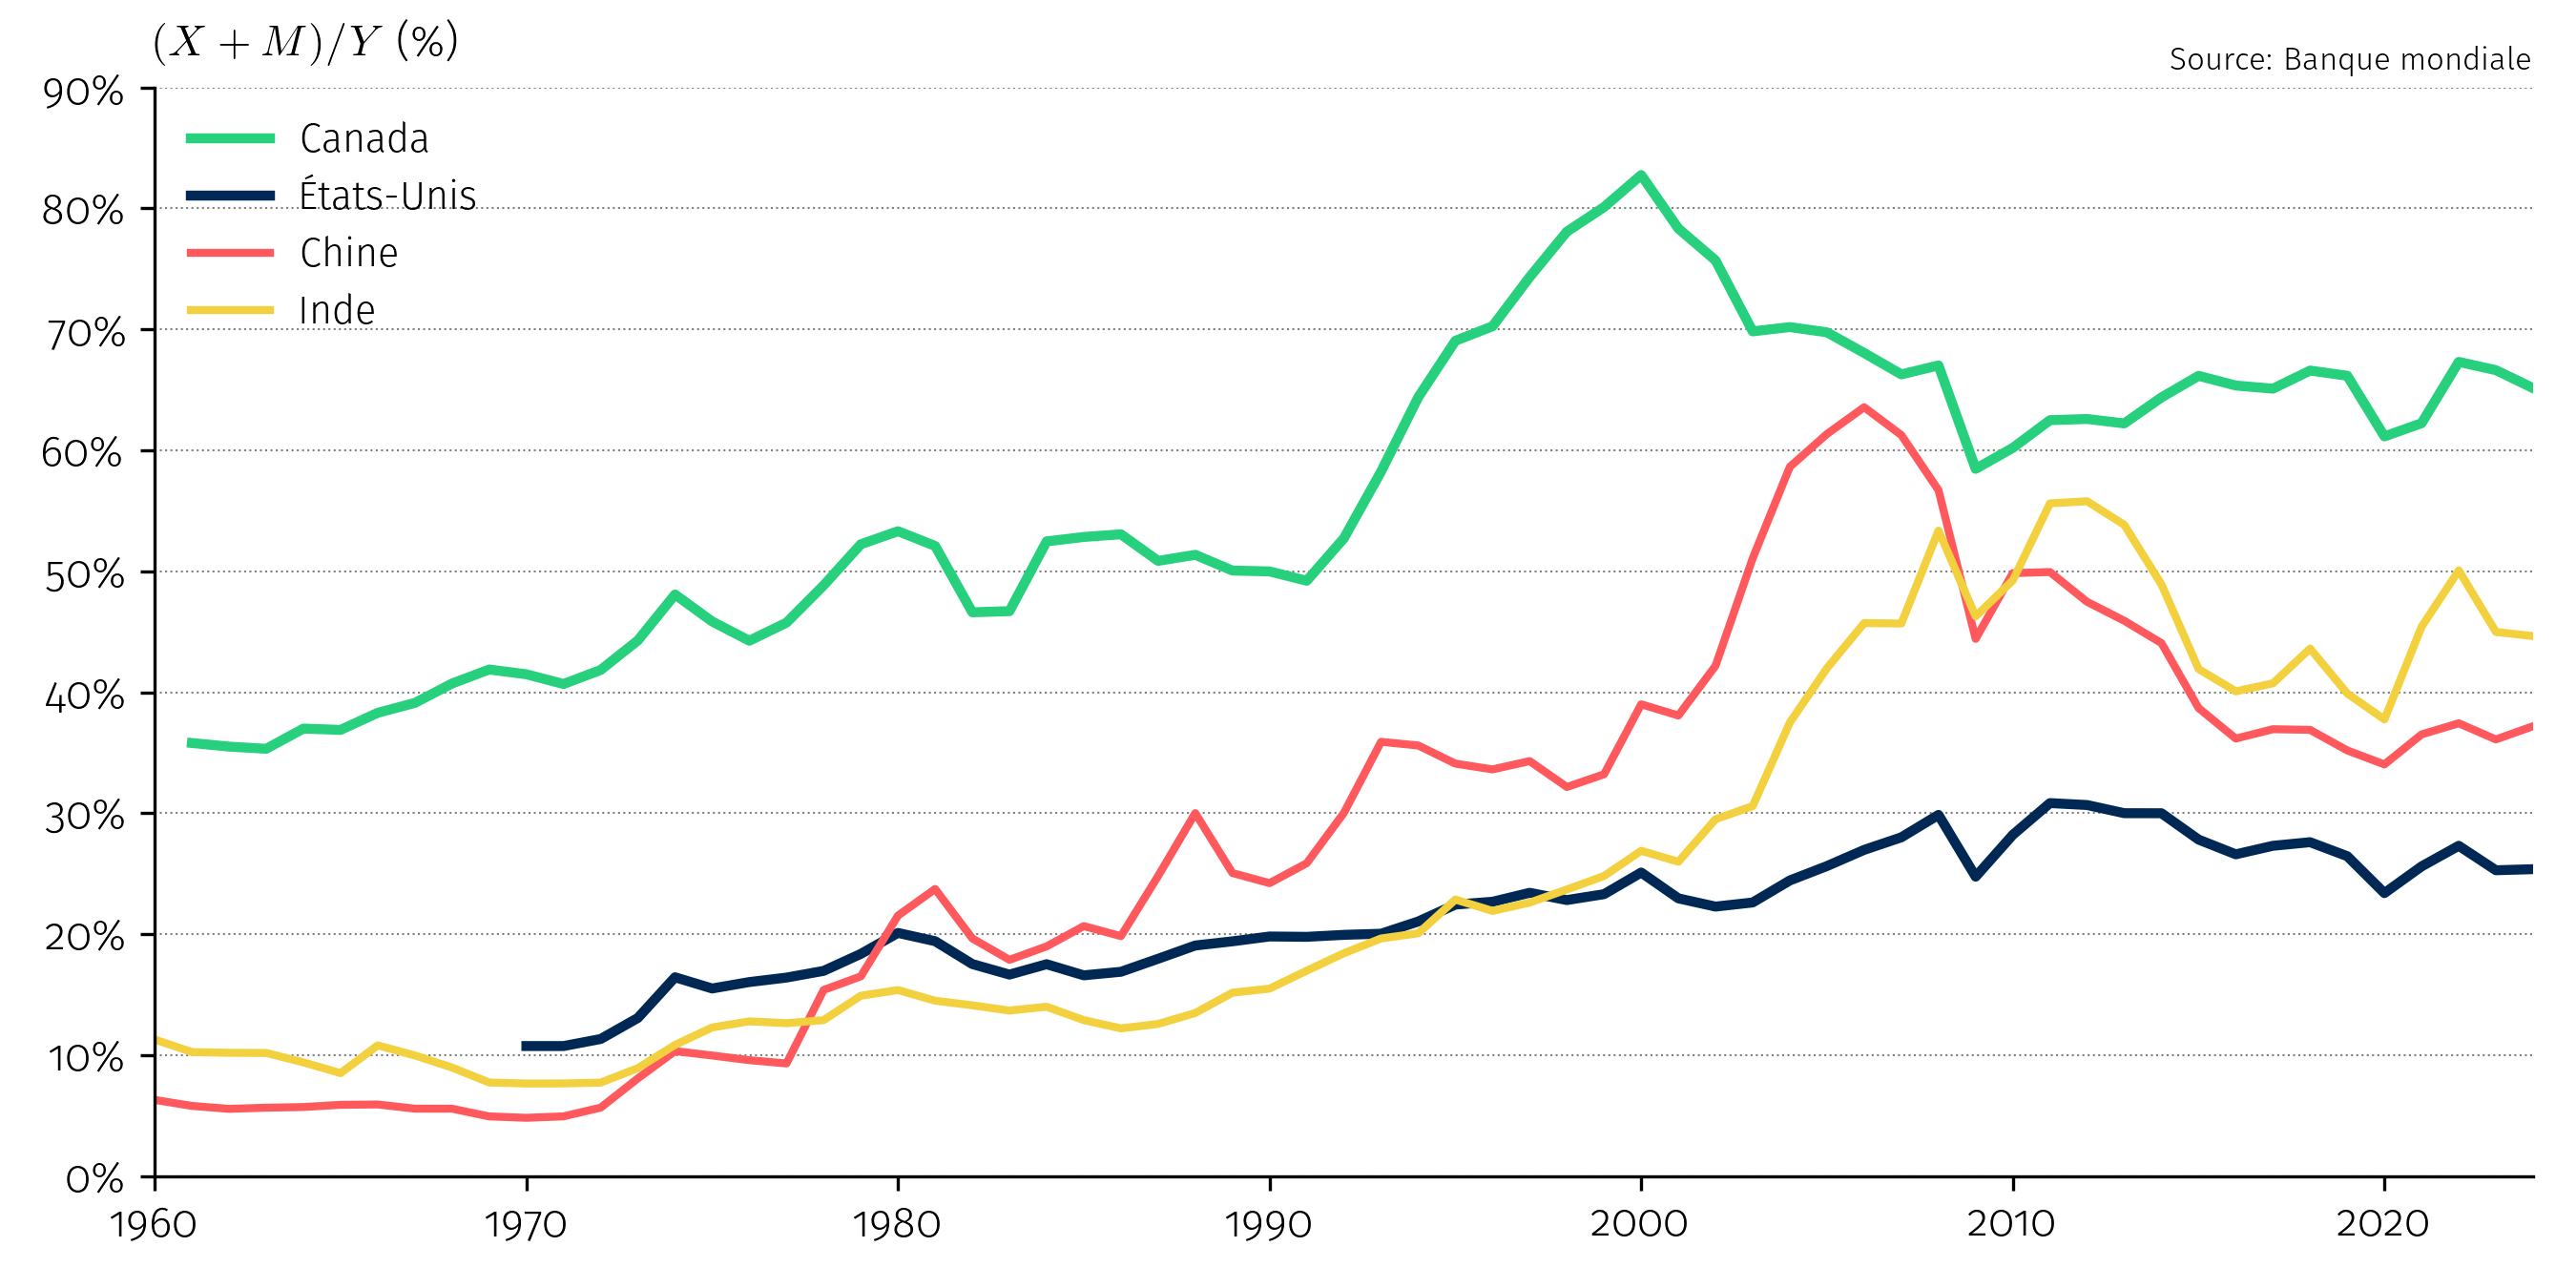
\includegraphics[width=0.95\textwidth, height=0.78\textheight, keepaspectratio]{trade_openness.png}
   \end{figure}
\end{frame}

\begin{frame}[t]{Pourquoi un recul\,?}
   \small
   \textbf{Quatre forces derrière le repli de la mondialisation :}
   \vspace{0.2cm}
   \begin{enumerate}
      \setlength\itemsep{0.25cm}
      \item \textbf{Inégalités et pertes d'emplois} dans les pays riches $\to$ opposition politique
      \item \textbf{Déficits commerciaux persistants} --- obsession politique, surtout aux É.-U.\
      \item \textbf{Vulnérabilité des chaînes d'approvisionnement} --- pandémie, géopolitique
      \item \textbf{Rivalité stratégique É.-U./Chine} --- technologie, sécurité nationale
   \end{enumerate}
   \vspace{0.15cm}
   \begin{bizimplication}
      La mondialisation n'est plus un acquis. Il faut diversifier les marchés, sécuriser les approvisionnements et anticiper les barrières tarifaires.
   \end{bizimplication}
\end{frame}

\begin{frame}{Trois questions pour cette séance}
   \vspace{0.5cm}
   \begin{enumerate}
      \setlength\itemsep{0.6cm}
      \item Qu'est-ce qui \textbf{détermine} les échanges commerciaux\,?
      \item D'où \textbf{viennent} les déficits commerciaux\,?
      \item Les droits de douane peuvent-ils \textbf{corriger} un déficit\,?
   \end{enumerate}
\end{frame}

% ============================================================================

\begin{frame}{Plan}
   \begin{enumerate}
      \setlength\itemsep{0.4cm}
      \item {\color{gray!50}La mondialisation en question}
      \item \textbf{D'où viennent les déficits commerciaux\,?}
      \item Le modèle épargne-investissement
      \item Le puzzle américain et l'excès d'épargne mondiale
      \item Les tarifs corrigent-ils le déficit\,?
      \item Géoéconomie : au-delà du modèle standard
      \item Récapitulatif du cours
   \end{enumerate}
\end{frame}

% ============================================================================
\sectionframe{D'où viennent les déficits commerciaux\,?}
% ============================================================================

\begin{frame}{Le compte courant américain}
   \begin{figure}
      \centering
      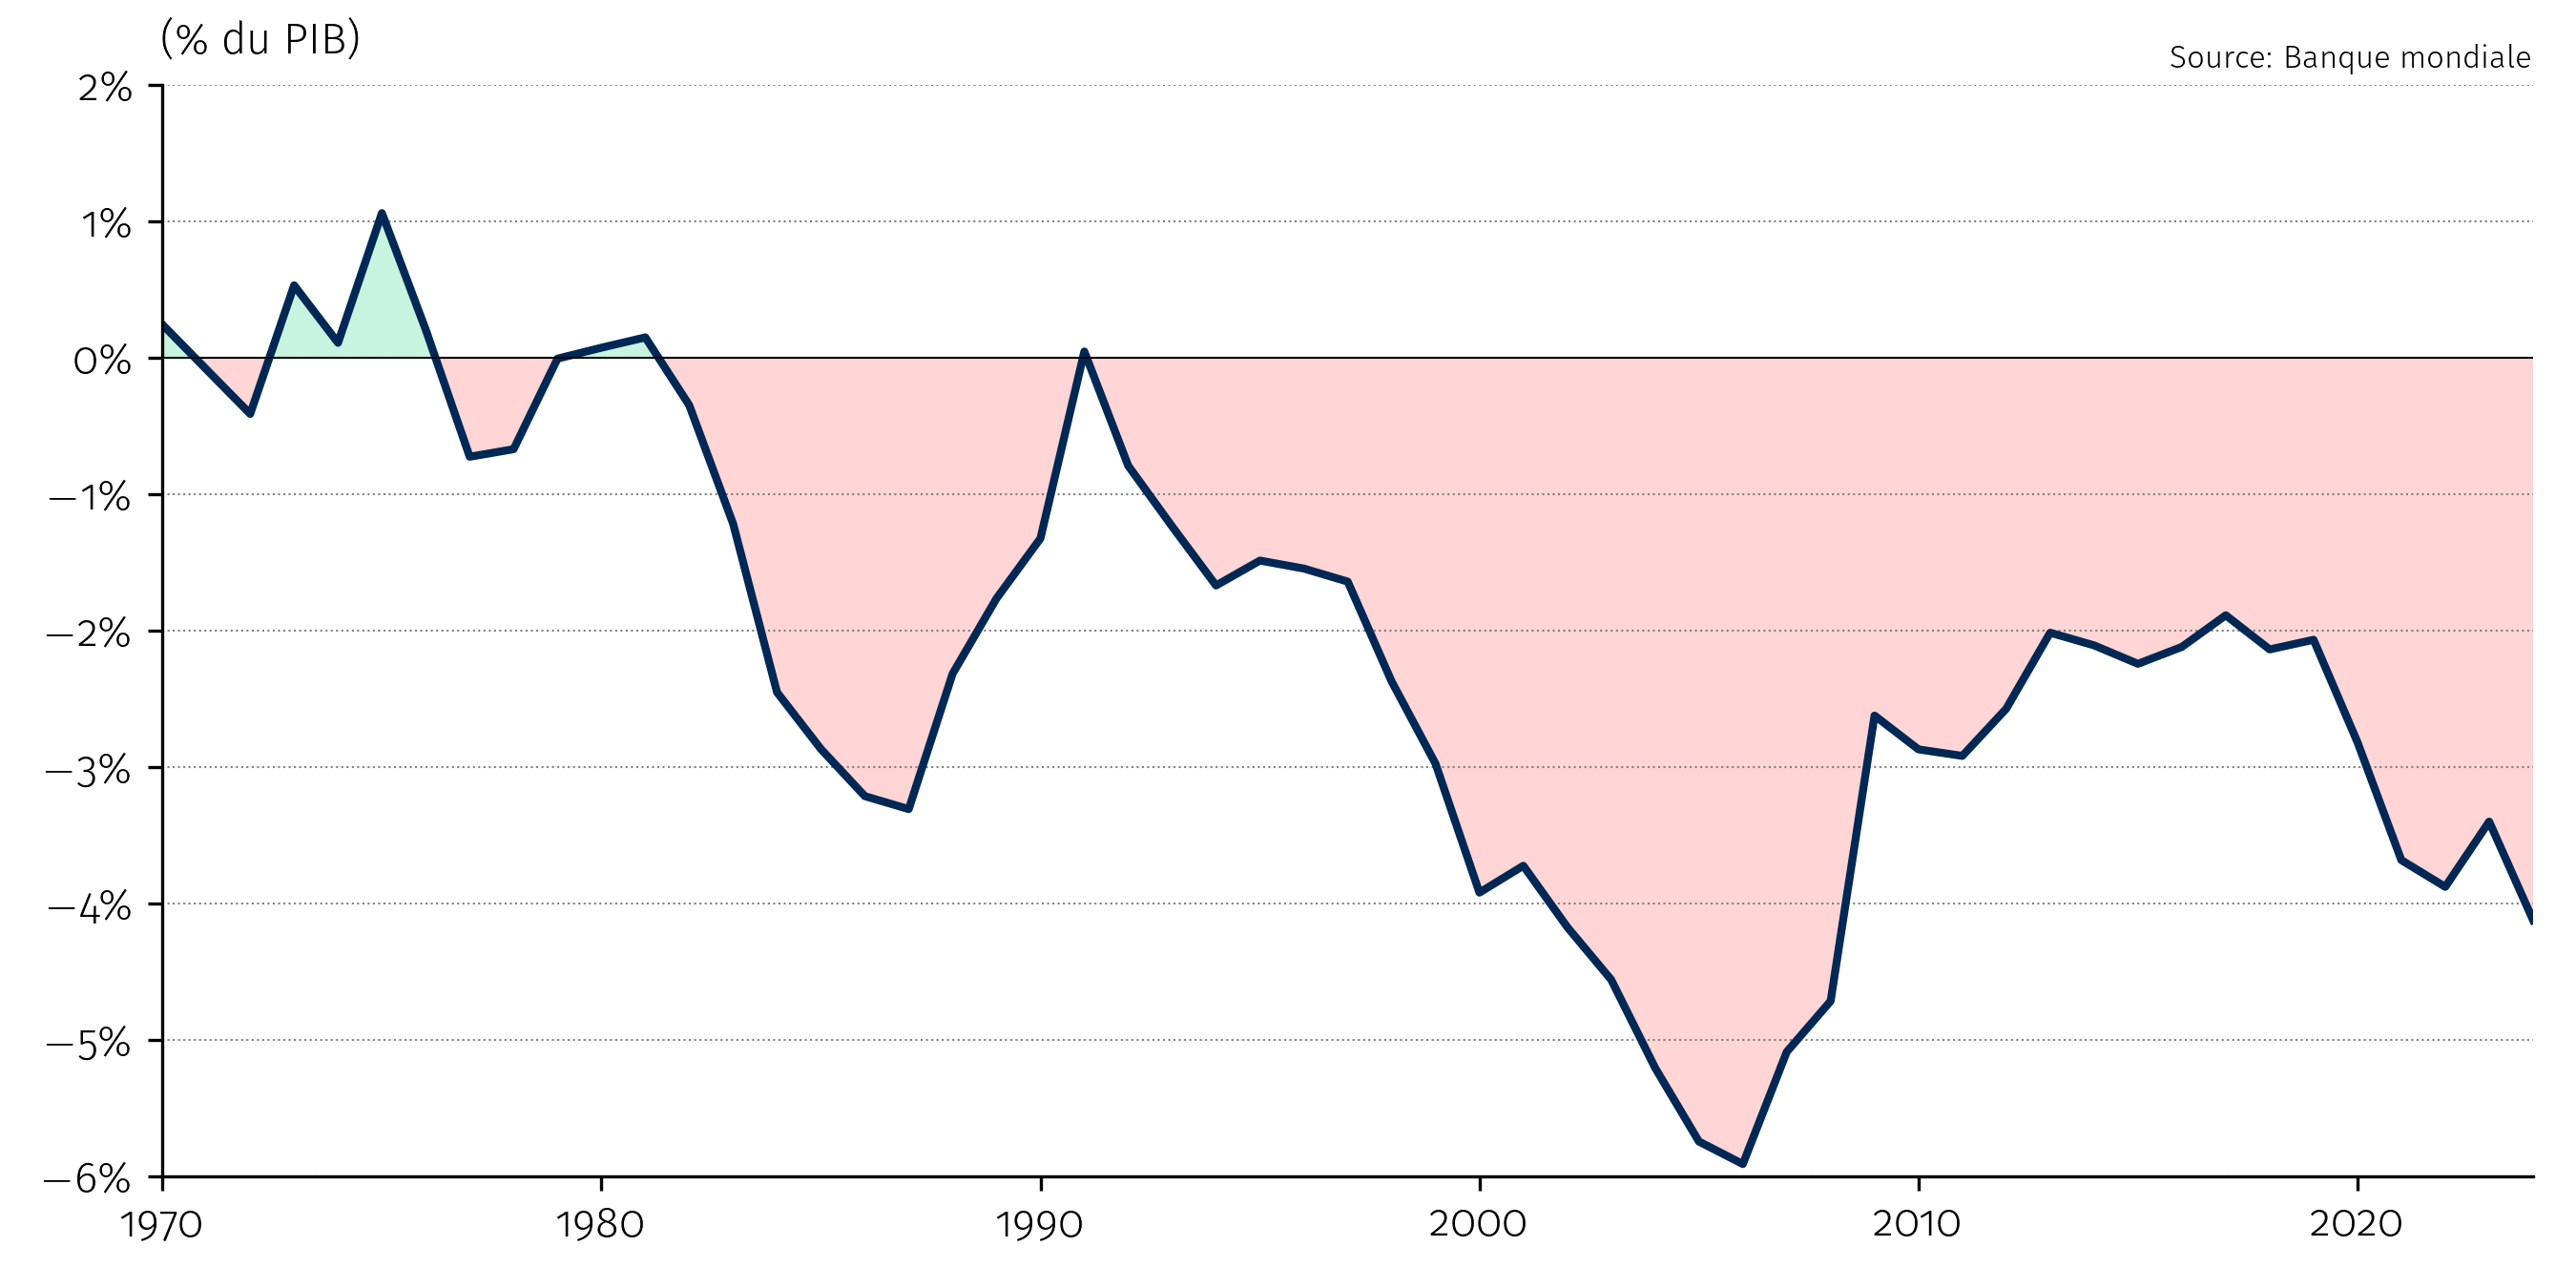
\includegraphics[width=0.95\textwidth, height=0.78\textheight, keepaspectratio]{us_ca_balance_gdp.png}
   \end{figure}
\end{frame}

\begin{frame}[t]{Du PIB au compte courant}
   \vspace{0.3cm}
   Partons de l'identité comptable du PIB (rappel séance 1) :
   \vspace{0.5cm}
   \begin{align*}
      Y &= C + I + G + NX \\[10pt]
      \underbrace{Y - C - G}_{\textcolor{HECgreen}{\boldsymbol{S}}} &= I + NX \\[14pt]
      \textcolor{HECgreen}{S} - I &= NX \approx CA
   \end{align*}
   \vspace{0.2cm}
   \centering
   où $\textcolor{HECgreen}{S = Y - C - G}$ est l'\textbf{épargne nationale} : ce qui reste du revenu\\
   après la consommation privée ($C$) et publique ($G$).
\end{frame}

\begin{frame}[t]{L'identité fondamentale}
   \vspace{0.3cm}
   \centering
   {\LARGE $\mathbf{CA = S - I}$}
   \vspace{0.5cm}

   \begin{columns}[T]
      \begin{column}{0.47\textwidth}
         \centering
         \textcolor{HECgreen}{\large\bfseries $S > I$ $\to$ $CA > 0$}\\[8pt]
         \small
         Le pays épargne plus qu'il n'investit.\\[4pt]
         Il \textbf{prête} l'excédent au reste du monde.\\[4pt]
         \textcolor{HECgray}{Ex.\ : Allemagne, Chine, Japon}
      \end{column}
      \begin{column}{0.47\textwidth}
         \centering
         \textcolor{HECcoral}{\large\bfseries $S < I$ $\to$ $CA < 0$}\\[8pt]
         \small
         Le pays investit plus qu'il n'épargne.\\[4pt]
         Il \textbf{emprunte} au reste du monde.\\[4pt]
         \textcolor{HECgray}{Ex.\ : É.-U., Canada, Australie}
      \end{column}
   \end{columns}
   \vspace{0.3cm}
   \begin{keyinsight}
      Le compte courant n'est pas une question de compétitivité internationale --- c'est l'\textbf{écart} entre épargne et investissement domestiques.
   \end{keyinsight}
\end{frame}

\begin{frame}[t]{Deux composantes de l'épargne : $S = S_P + S_G$}
   \vspace{0.1cm}
   \begin{columns}[T]
      \begin{column}{0.47\textwidth}
         \begin{defbox}[Épargne privée ($S_P$)]
            \footnotesize
            Ménages + entreprises.\\[4pt]
            \textbf{Déterminants :}
            \begin{itemize}
               \setlength\itemsep{0.08cm}
               \item Taux d'intérêt ($r$)
               \item Revenu courant
               \item Richesse et incertitude
               \item Accès au crédit
            \end{itemize}
         \end{defbox}
      \end{column}
      \begin{column}{0.47\textwidth}
         \begin{defbox}[Épargne publique ($S_G$)]
            \footnotesize
            $S_G = T - G$\\[4pt]
            \textbf{Déterminants :}
            \begin{itemize}
               \setlength\itemsep{0.08cm}
               \item Recettes fiscales ($T$)
               \item Dépenses publiques ($G$)
               \item $S_G > 0$ : surplus budgétaire
               \item $S_G < 0$ : déficit budgétaire
            \end{itemize}
         \end{defbox}
      \end{column}
   \end{columns}
\end{frame}

\begin{frame}[t]{Les déficits jumeaux}
   \small
   Puisque $S = S_P + S_G$, on peut écrire :
   \vspace{0.1cm}
   \[CA = S_P + S_G - I\]
   \vspace{0.1cm}
   Si $S_P$ et $I$ ne changent pas, un creusement du déficit budgétaire ($S_G \downarrow$) se traduit par un creusement du déficit commercial ($CA \downarrow$).
   \vspace{0.25cm}
   \begin{warning}[Déficits jumeaux]
      Un pays qui creuse son déficit \textbf{budgétaire} creuse aussi son déficit \textbf{commercial}.
   \end{warning}
   \vspace{0.25cm}
   \textbf{Exemple :} les É.-U.\ sous Reagan (années 1980). Baisses d'impôts massives + hausse des dépenses militaires $\to$ $S_G \downarrow$ $\to$ déficit budgétaire \textbf{et} déficit commercial records.
\end{frame}

\begin{frame}{Les déficits jumeaux américains}
   \begin{figure}
      \centering
      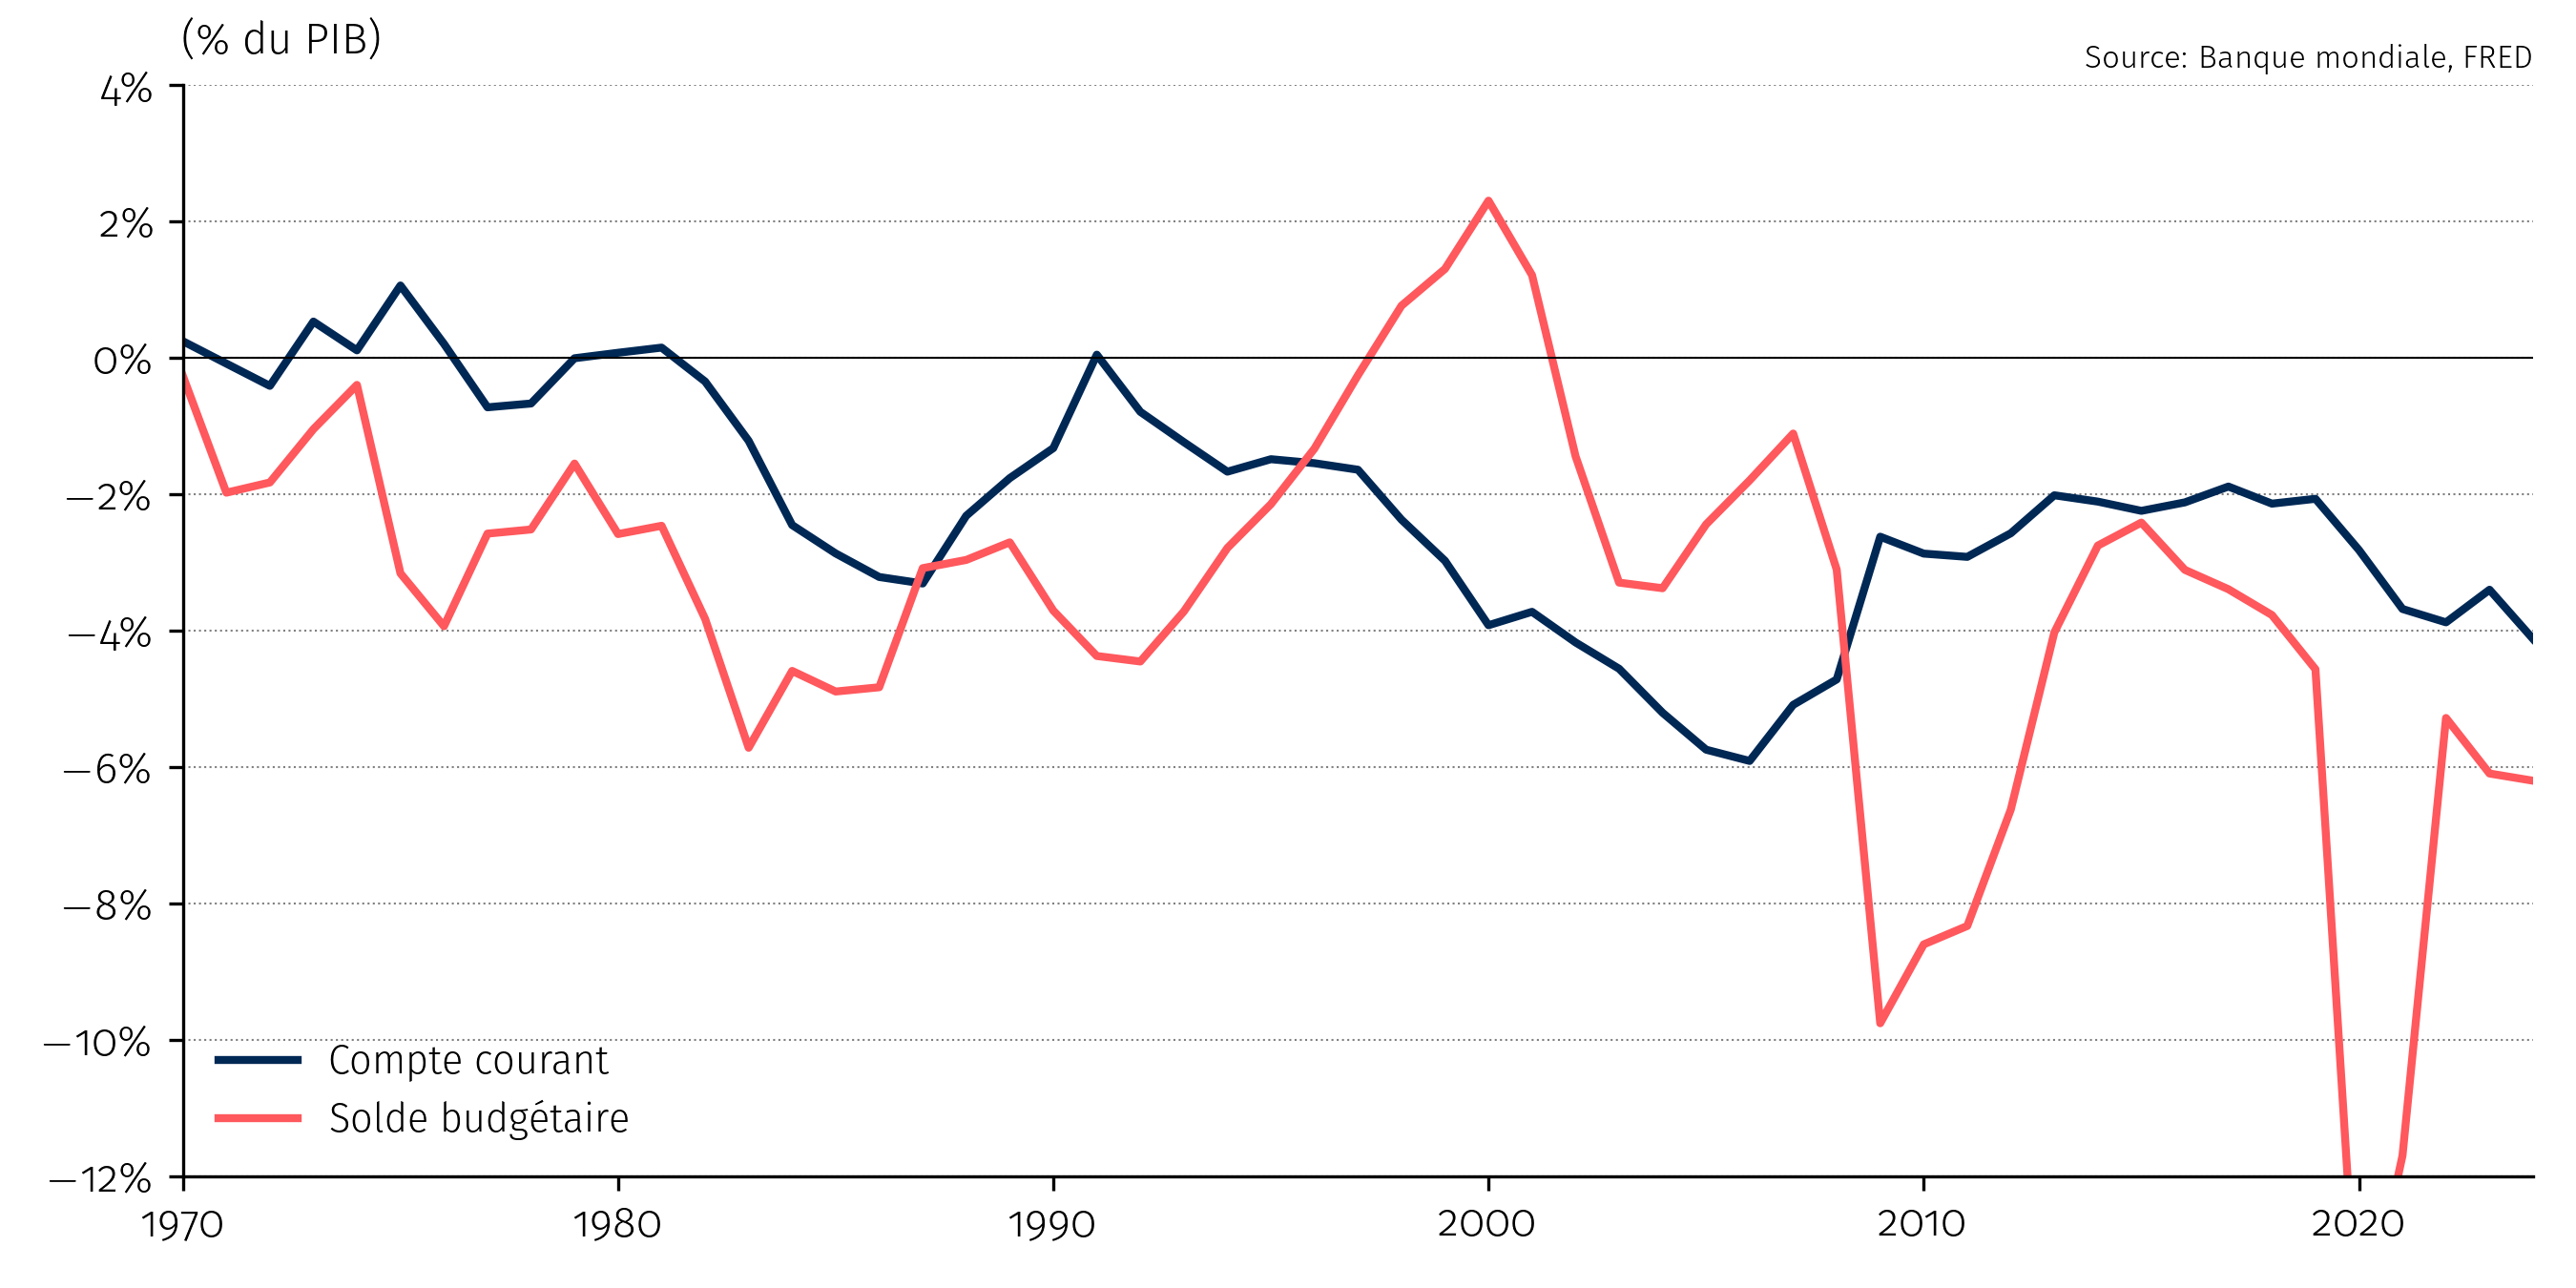
\includegraphics[width=0.95\textwidth, height=0.78\textheight, keepaspectratio]{us_twin_deficits.png}
   \end{figure}
\end{frame}

\begin{frame}[t]{Où en sommes-nous\,?}
   \vspace{0.3cm}
   Nous savons maintenant que $CA = S - I$.
   \vspace{0.3cm}
   \begin{itemize}
      \setlength\itemsep{0.3cm}
      \item Le déficit commercial américain reflète un \textbf{écart} entre épargne et investissement, pas un manque de compétitivité
      \item La prochaine étape : un \textbf{modèle} qui détermine $S$, $I$ et le taux d'intérêt en économie ouverte
   \end{itemize}
   \vspace{0.3cm}
   \begin{warning}[À garder en tête]
      Si $CA = S - I$, les droits de douane peuvent-ils \textbf{vraiment} corriger un déficit\,? Nous y reviendrons.
   \end{warning}
\end{frame}

% ============================================================================

\begin{frame}{Plan}
   \begin{enumerate}
      \setlength\itemsep{0.4cm}
      \item {\color{gray!50}La mondialisation en question}
      \item {\color{gray!50}D'où viennent les déficits commerciaux\,?}
      \item \textbf{Le modèle épargne-investissement}
      \item Le puzzle américain et l'excès d'épargne mondiale
      \item Les tarifs corrigent-ils le déficit\,?
      \item Géoéconomie : au-delà du modèle standard
      \item Récapitulatif du cours
   \end{enumerate}
\end{frame}

% ============================================================================
\sectionframe{Le modèle épargne-investissement}
% ============================================================================

\begin{frame}[t]{La courbe d'épargne}
   \begin{columns}[T]
      \begin{column}{0.50\textwidth}
         \centering
         % S curve: r = 0.75q → passes through origin (0, 0)
         \begin{tikzpicture}[scale=0.9]
            % S curve (upward sloping — higher r → more saving)
            \draw[very thick, HECnavy] (0,0) -- (5.5,4.125)
               node[right, curvelabel, text=HECnavy] {$S(r)$};
            % Axes (drawn last for z-order)
            \draw[econaxis] (0,0) -- (6.5,0) node[right] {$S, I$};
            \draw[econaxis] (0,0) -- (0,4.5) node[above] {$r$};
         \end{tikzpicture}
      \end{column}
      \begin{column}{0.45\textwidth}
         \small
         \vspace{0.3cm}
         \textbf{Pourquoi la pente positive\,?}
         \vspace{0.2cm}
         \begin{itemize}
            \setlength\itemsep{0.2cm}
            \item $r \uparrow$ $\to$ rendement de l'épargne $\uparrow$ $\to$ les ménages épargnent davantage
         \end{itemize}
         \vspace{0.3cm}
         \textbf{Autres déterminants} (déplacements) :
         \vspace{0.1cm}
         \begin{itemize}
            \setlength\itemsep{0.12cm}
            \item Revenu, confiance
            \item Démographie (âge)
            \item Politique budgétaire ($T$, $G$)
         \end{itemize}
      \end{column}
   \end{columns}
\end{frame}

\begin{frame}[t]{La courbe d'investissement}
   \begin{columns}[T]
      \begin{column}{0.50\textwidth}
         \centering
         % I curve: r = -0.75q + 4.5 → y-intercept (0, 4.5), x-intercept (6.0, 0)
         \begin{tikzpicture}[scale=0.9]
            % I curve (downward sloping — higher r → less investment)
            \draw[very thick, HECcoral] (0,4.5) -- (6.0,0)
               node[above, curvelabel, text=HECcoral] {$I(r)$};
            % Axes (drawn last for z-order)
            \draw[econaxis] (0,0) -- (6.5,0) node[right] {$S, I$};
            \draw[econaxis] (0,0) -- (0,4.8) node[above] {$r$};
         \end{tikzpicture}
      \end{column}
      \begin{column}{0.45\textwidth}
         \small
         \vspace{0.3cm}
         \textbf{Pourquoi la pente négative\,?}
         \vspace{0.2cm}
         \begin{itemize}
            \setlength\itemsep{0.2cm}
            \item $r \uparrow$ $\to$ coût du capital $\uparrow$ $\to$ moins de projets rentables
         \end{itemize}
         \vspace{0.3cm}
         \textbf{Autres déterminants} (déplacements) :
         \vspace{0.1cm}
         \begin{itemize}
            \setlength\itemsep{0.12cm}
            \item Productivité ($A$), technologie
            \item Optimisme des entreprises
            \item Incertitude, réglementation
         \end{itemize}
      \end{column}
   \end{columns}
\end{frame}

\begin{frame}{Équilibre en économie fermée}
   \centering
   % S curve: r = 0.75q → passes through origin (0, 0)
   % I curve: r = -0.75q + 4.5 → y-intercept (0, 4.5), x-intercept (6.0, 0)
   % Equilibrium: 0.75q = -0.75q + 4.5 → 1.5q = 4.5 → q = 3.0, r = 2.25
   \begin{tikzpicture}[scale=1]
      % Reference lines to axes
      \draw[refline] (3.0,0) node[below, pointlabel] {$S^* = I^*$} -- (3.0,2.25);
      \draw[refline] (0,2.25) node[left, pointlabel] {$r^*$} -- (3.0,2.25);
      % S curve (HECnavy, upward)
      \draw[very thick, HECnavy] (0,0) -- (5.5,4.125)
         node[right, curvelabel, text=HECnavy] {$S$};
      % I curve (HECcoral, downward)
      \draw[very thick, HECcoral] (0,4.5) -- (6.0,0)
         node[above, curvelabel, text=HECcoral] {$I$};
      % Equilibrium
      \filldraw[eqpoint=HECnavy] (3.0,2.25) circle (3pt);
      \node[pointlabel, HECnavy, above] at (3.0,2.25) {$E_0$};
      % Axes (drawn last for z-order)
      \draw[econaxis] (0,0) -- (6.5,0) node[right] {$S, I$};
      \draw[econaxis] (0,0) -- (0,4.8) node[above] {$r$};
   \end{tikzpicture}
\end{frame}

\begin{frame}[t]{Application --- les baby-boomers prennent leur retraite}
   \begin{columns}[T]
      \begin{column}{0.52\textwidth}
         \centering
         % S shifts LEFT: retirees dissave → less national saving
         % Original S: r = 0.75q → passes through origin (0, 0)
         % New S': r = 0.75q + 1.2 → y-intercept (0, 1.2)
         % I: r = -0.75q + 4.5 → y-intercept (0, 4.5), x-intercept (6.0, 0)
         % New eq with I: 0.75q + 1.2 = -0.75q + 4.5 → q = 2.2, r = 2.85
         \begin{tikzpicture}[scale=0.9]
            % Reference lines
            \draw[refline] (3.0,0) node[below, pointlabel] {$S_0^*$} -- (3.0,2.25);
            \draw[refline] (0,2.25) node[left, pointlabel] {$r_0^*$} -- (3.0,2.25);
            \draw[refline, HECgreen] (2.2,0) node[below, pointlabel, text=HECgreen] {$S_1^*$} -- (2.2,2.85);
            \draw[refline, HECgreen] (0,2.85) node[left, pointlabel, text=HECgreen] {$r_1^*$} -- (2.2,2.85);
            % Original S (dashed gray)
            \draw[original] (0,0) -- (5.5,4.125)
               node[right, curvelabel, text=HECgray] {$S$};
            % New S' (shifted left, HECgreen)
            \draw[curveshift, HECgreen] (0,1.2) -- (4.3,4.425)
               node[right, curvelabel, text=HECgreen] {$S'$};
            % I curve (unchanged)
            \draw[very thick, HECcoral] (0,4.5) -- (6.0,0)
               node[above, curvelabel, text=HECcoral] {$I$};
            % Shift arrow (leftward on S) — at r=3.0: S at q=4.0, S' at q=2.4
            \draw[shiftarrow, HECgreen] (3.8,3.0) -- (2.6,3.0);
            % Original equilibrium (faded)
            \filldraw[eqfaded] (3.0,2.25) circle (2.5pt);
            \node[pointlabel, HECgray, right] at (3.0,2.25) {$E_0$};
            % New equilibrium
            \filldraw[eqpoint=HECgreen] (2.2,2.85) circle (3pt);
            \node[pointlabel, HECgreen, above] at (2.2,2.85) {$E_1$};
            % Axes (drawn last for z-order)
            \draw[econaxis] (0,0) -- (6.5,0) node[right] {$S, I$};
            \draw[econaxis] (0,0) -- (0,4.8) node[above] {$r$};
         \end{tikzpicture}
      \end{column}
      \begin{column}{0.45\textwidth}
         \small
         \vspace{0.2cm}
         \textbf{Le vieillissement réduit l'épargne :}
         \vspace{0.2cm}
         \begin{itemize}
            \setlength\itemsep{0.15cm}
            \item Les retraités \textbf{désépargnent}
            \item $S$ se déplace vers la \textbf{gauche}
            \item $r^* \uparrow$ et $S^* = I^* \downarrow$
         \end{itemize}
         \vspace{0.2cm}
         \begin{keyinsight}
            Le vieillissement hausse les taux d'intérêt. En économie ouverte, cette baisse d'épargne se traduirait aussi par un \textbf{déficit commercial}.
         \end{keyinsight}
      \end{column}
   \end{columns}
\end{frame}

\begin{frame}[t]{Application --- boom d'investissement (e.g., IA et centre de données)}
   \begin{columns}[T]
      \begin{column}{0.52\textwidth}
         \centering
         % I shifts RIGHT: new investment opportunities
         % S: r = 0.75q → passes through origin (0, 0)
         % Original I: r = -0.75q + 4.5 → y-intercept (0, 4.5), x-intercept (6.0, 0)
         % New I': r = -0.75q + 5.7 → y-intercept (0, 5.7), x-intercept (7.6, 0)
         % New eq with S: 0.75q = -0.75q + 5.7 → q = 3.8, r = 2.85
         % Match the previous slide's physical chart footprint
         \begin{tikzpicture}[x=0.75cm, y=0.72cm]
            % Reference lines
            \draw[refline] (3.0,0) node[below, pointlabel] {$I_0^*$} -- (3.0,2.25);
            \draw[refline] (0,2.25) node[left, pointlabel] {$r_0^*$} -- (3.0,2.25);
            \draw[refline, HECgreen] (3.8,0) node[below, pointlabel, text=HECgreen] {$I_1^*$} -- (3.8,2.85);
            \draw[refline, HECgreen] (0,2.85) node[left, pointlabel, text=HECgreen] {$r_1^*$} -- (3.8,2.85);
            % S curve (unchanged)
            \draw[very thick, HECnavy] (0,0) -- (6.8,5.1)
               node[right, curvelabel, text=HECnavy] {$S$};
            % Original I (dashed gray)
            \draw[original] (0,4.5) -- (6.0,0)
               node[above, curvelabel, text=HECgray] {$I$};
            % New I' (shifted right, HECgreen)
            \draw[curveshift, HECgreen] (0,5.7) -- (7.0,0.45)
               node[above, curvelabel, text=HECgreen] {$I'$};
            % Shift arrow (rightward on I) — at r=3.5: I at q=1.33, I' at q=2.93
            \draw[shiftarrow, HECgreen] (1.5,3.5) -- (2.8,3.5);
            % Original equilibrium (faded)
            \filldraw[eqfaded] (3.0,2.25) circle (2.5pt);
            \node[pointlabel, HECgray, above] at (3.0,2.25) {$E_0$};
            % New equilibrium
            \filldraw[eqpoint=HECgreen] (3.8,2.85) circle (3pt);
            \node[pointlabel, HECgreen, right] at (3.8,2.85) {$E_1$};
            % Axes (drawn last for z-order)
            \draw[econaxis] (0,0) -- (7.8,0) node[right] {$S, I$};
            \draw[econaxis] (0,0) -- (0,6.0) node[above] {$r$};
         \end{tikzpicture}
      \end{column}
      \begin{column}{0.45\textwidth}
         \small
         \vspace{0.2cm}
         \textbf{Nouvelles opportunités d'investissement :}
         \vspace{0.15cm}
         \begin{itemize}
            \setlength\itemsep{0.1cm}
            \item IA, énergie verte $\to$ plus de projets rentables
            \item $I$ se déplace vers la \textbf{droite}
            \item $r^* \uparrow$ et $S^* = I^* \uparrow$
         \end{itemize}
         \vspace{0.1cm}
         \begin{bizimplication}
            \footnotesize
            Si l'IA augmente $I$, les taux resteront élevés. En économie ouverte, ce boom attire des capitaux étrangers et creuse le \textbf{déficit du CA}.
         \end{bizimplication}
      \end{column}
   \end{columns}
\end{frame}

\begin{frame}[t]{Les marchés de capitaux sont mondiaux}
   \small
   \vspace{0.1cm}
   Une entreprise canadienne qui veut construire une usine n'a pas besoin de compter sur l'épargne canadienne. Elle peut emprunter à un \textbf{fonds de pension} allemand, un \textbf{fonds souverain} norvégien ou une \textbf{banque} japonaise.
   \vspace{0.2cm}

   Il existe donc un \textbf{taux d'intérêt mondial} $r^w$ auquel les pays peuvent emprunter ou prêter sur les marchés internationaux.
   \vspace{0.15cm}
   \begin{itemize}
      \setlength\itemsep{0.15cm}
      \item Si $r^w < r^*$ $\to$ moins cher d'emprunter à l'étranger $\to$ capitaux entrants $\to$ $I > S$
      \item Si $r^w > r^*$ $\to$ plus rentable de prêter à l'étranger $\to$ capitaux sortants $\to$ $S > I$
   \end{itemize}
   \vspace{0.15cm}
   \begin{bizimplication}
      \footnotesize
      Pour une entreprise canadienne, le coût du capital n'est pas déterminé uniquement par l'épargne canadienne --- il dépend des conditions financières \textbf{mondiales}.
   \end{bizimplication}
\end{frame}

\begin{frame}[t]{De l'économie fermée à l'économie ouverte}
   \small
   \vspace{0.1cm}
   \begin{columns}[T]
      \begin{column}{0.47\textwidth}
         \textbf{\textcolor{HECgray}{Économie fermée}}
         \vspace{0.2cm}
         \begin{itemize}
            \setlength\itemsep{0.2cm}
            \item $S = I$ toujours
            \item Pas d'emprunt possible à l'étranger
            \item $r$ s'ajuste pour égaliser $S$ et $I$
         \end{itemize}
      \end{column}
      \begin{column}{0.47\textwidth}
         \textbf{\textcolor{HECnavy}{Économie ouverte}}
         \vspace{0.2cm}
         \begin{itemize}
            \setlength\itemsep{0.2cm}
            \item $S \neq I$ est possible
            \item La différence est le compte courant
            \item $CA = S - I$
         \end{itemize}
      \end{column}
   \end{columns}
   \vspace{0.3cm}
   \begin{defbox}[Petite vs grande économie ouverte]
      \footnotesize
      \textbf{Grande économie ouverte} (É.-U., Chine) : ses décisions affectent $r^w$. Un choc domestique modifie partiellement le taux mondial.\\[4pt]
      \textbf{Petite économie ouverte} (Canada, Suisse) : $r^w$ est \textbf{donné}. Les politiques domestiques affectent le compte courant, pas le taux d'intérêt.
   \end{defbox}
\end{frame}

\begin{frame}[t]{Diagramme S-I en économie ouverte}
   \centering
   % S curve: r = 0.75q → passes through origin (0, 0)
   % I curve: r = -0.75q + 4.5 → y-intercept (0, 4.5), x-intercept (6.0, 0)
   % Closed eq: q=3.0, r=2.25
   % World rate: r^w = 1.8 (below closed eq → domestic I > S → deficit)
   % At r^w=1.8: S(1.8) = 1.8/0.75 = 2.4, I(1.8) = (4.5-1.8)/0.75 = 3.6
   % CA = S - I = 2.4 - 3.6 = -1.2 (deficit)
   \begin{tikzpicture}[scale=1]
      % World interest rate (horizontal)
      \draw[HECgreen, very thick, dotted] (0,1.8) -- (6.5,1.8)
         node[right, curvelabel, text=HECgreen] {$r^w$};
      % Reference lines at r^w
      \draw[refline] (2.4,0) node[below, pointlabel] {$S$} -- (2.4,1.8);
      \draw[refline] (3.6,0) node[below, pointlabel] {$I$} -- (3.6,1.8);
      % S curve (HECnavy, upward)
      \draw[very thick, HECnavy] (0,0) -- (5.5,4.125)
         node[right, curvelabel, text=HECnavy] {$S$};
      % I curve (HECcoral, downward)
      \draw[very thick, HECcoral] (0,4.5) -- (6.0,0)
         node[above, curvelabel, text=HECcoral] {$I$};
      % Open-economy allocations at r^w
      \filldraw[eqpoint=HECnavy] (2.4,1.8) circle (2.7pt);
      \filldraw[eqpoint=HECcoral] (3.6,1.8) circle (2.7pt);
      % CA deficit brace
      \draw[decorate, decoration={brace, amplitude=8pt, mirror}, very thick, HECcoral]
         (2.4,-0.55) -- (3.6,-0.55)
         node[midway, below=8pt, font=\small\bfseries, text=HECcoral] {$CA < 0$ (déficit)}
         node[midway, below=20pt, font=\scriptsize, text=HECcoral] {Le pays emprunte au reste du monde};
      % Axes (drawn last for z-order)
      \draw[econaxis] (0,0) -- (6.5,0) node[right] {$S, I$};
      \draw[econaxis] (0,0) -- (0,4.8) node[above] {$r$};
   \end{tikzpicture}
\end{frame}

\begin{frame}[t]{Le diagramme à deux panneaux}
   \centering
   \vfill
   % Panel 1 (World): S^w: r = 0.42q + 0.13, I^w: r = -0.65q + 4.42
   %   Equilibrium: 0.42q + 0.13 = -0.65q + 4.42 → 1.07q = 4.29 → q = 4.01, r = 1.82 ≈ 1.8
   % Panel 2 (Domestic): S_H: r = 0.75q, I_H: r = -0.75q + 4.5
   %   At r^w = 1.8: S_H = 2.4, I_H = 3.6, CA = -1.2
   \begin{tikzpicture}[scale=0.9]
      % ── Panel 1: World ──────────────────────────
      \begin{scope}[xshift=0cm]
         \node[font=\normalsize\bfseries, text=HECnavy] at (3.25,5.2) {Monde};
         % r^w horizontal (green dotted, spans full width)
         \draw[HECgreen, very thick, dotted] (0,1.8) -- (6.5,1.8);
         % S^w: r = 0.42q + 0.13
         \draw[very thick, HECnavy] (0,0.13) -- (6.0,2.65)
            node[above, xshift=-4pt, curvelabel, text=HECnavy] {$S^w$};
         % I^w: r = -0.65q + 4.42
         \draw[very thick, HECcoral] (0,4.42) -- (6.0,0.52)
            node[above, xshift=-2pt, curvelabel, text=HECcoral] {$I^w$};
         % Equilibrium
         \draw[refline] (4.01,0) node[below, pointlabel] {$S^w = I^w$} -- (4.01,1.8);
         \node[left, pointlabel] at (0,1.8) {$r^w$};
         \filldraw[eqpoint=HECgreen] (4.01,1.8) circle (3pt);
         \node[pointlabel, HECgreen, above right] at (4.01,1.8) {$E^w$};
         % Axes
         \draw[econaxis] (0,0) -- (6.5,0) node[right] {$S, I$};
         \draw[econaxis] (0,0) -- (0,4.8) node[above] {$r$};
      \end{scope}

      % ── Panel 2: Domestic ──────────────────────
      \begin{scope}[xshift=7.5cm]
         \node[font=\normalsize\bfseries, text=HECnavy] at (3.0,5.2) {Domestique};
         % r^w horizontal
         \draw[HECgreen, very thick, dotted] (0,1.8) -- (5.8,1.8);
         \node[left, pointlabel, text=HECgreen] at (0,1.8) {$r^w$};
         % S_H: r = 0.75q
         \draw[very thick, HECnavy] (0,0) -- (5.5,4.125)
            node[above left, curvelabel, text=HECnavy] {$S_H$};
         % I_H: r = -0.75q + 4.5
         \draw[very thick, HECcoral] (0,4.5) -- (6.0,0)
            node[above, curvelabel, text=HECcoral] {$I_H$};
         % Allocations at r^w
         \draw[refline] (2.4,0) node[below, pointlabel] {$S_H$} -- (2.4,1.8);
         \draw[refline] (3.6,0) node[below, pointlabel] {$I_H$} -- (3.6,1.8);
         \filldraw[eqpoint=HECnavy] (2.4,1.8) circle (2.7pt);
         \filldraw[eqpoint=HECcoral] (3.6,1.8) circle (2.7pt);
         % CA deficit brace
         \draw[decorate, decoration={brace, amplitude=8pt, mirror}, very thick, HECcoral]
            (2.4,-0.55) -- (3.6,-0.55)
            node[midway, below=8pt, font=\small\bfseries, text=HECcoral] {$CA < 0$};
         % Axes
         \draw[econaxis] (0,0) -- (6.2,0) node[right] {$S, I$};
         \draw[econaxis] (0,0) -- (0,4.8) node[above] {$r$};
      \end{scope}
   \end{tikzpicture}
   \vfill
\end{frame}


% ============================================================================

\begin{frame}{Plan}
   \begin{enumerate}
      \setlength\itemsep{0.4cm}
      \item {\color{gray!50}La mondialisation en question}
      \item {\color{gray!50}D'où viennent les déficits commerciaux\,?}
      \item {\color{gray!50}Le modèle épargne-investissement}
      \item \textbf{Le puzzle américain et l'excès d'épargne mondiale}
      \item Les tarifs corrigent-ils le déficit\,?
      \item Géoéconomie : au-delà du modèle standard
      \item Récapitulatif du cours
   \end{enumerate}
\end{frame}

% ============================================================================
\sectionframe{Le puzzle américain et l'excès\\ d'épargne mondiale}
% ============================================================================

\begin{frame}[t]{Le puzzle du déficit américain}
   \small
   \vspace{0.2cm}
   Depuis les années 1980, les É.-U.\ ont un \textbf{déficit persistant} du compte courant et des taux d'intérêt réels en \textbf{baisse}.
   \vspace{0.3cm}

   Testons trois hypothèses avec notre diagramme à deux panneaux :
   \vspace{0.15cm}
   \begin{enumerate}
      \setlength\itemsep{0.3cm}
      \item \textbf{Déficits budgétaires} ($S_G \downarrow$) --- baisse de l'épargne publique
      \item \textbf{Boom technologique} ($I \uparrow$) --- hausse de l'investissement
      \item \textbf{Excès d'épargne mondiale} ($S^w_R \uparrow$) --- hypothèse de Bernanke
   \end{enumerate}
   \vspace{0.2cm}
   \textbf{Laquelle peut expliquer à la fois $CA \downarrow$ et $r \downarrow$\,?}
\end{frame}

% --- Hypothèse 1: Déficits budgétaires ---

\begin{frame}[t]{Hypothèse 1 --- déficits budgétaires}
   \small
   \vspace{0.1cm}
   Les É.-U.\ accumulent des déficits budgétaires depuis les années 1980.
   \vspace{0.2cm}
   \begin{itemize}
      \setlength\itemsep{0.2cm}
      \item Baisses d'impôts Reagan (1981), Bush (2001, 2003), Trump (2017)
      \item Guerres en Irak et Afghanistan, plans de relance
      \item $S_G \downarrow$ $\to$ $S = S_P + S_G$ diminue $\to$ $S_H$ se déplace vers la \textbf{gauche}
   \end{itemize}
   \vspace{0.15cm}
   \textbf{Que prédit le modèle\,?}
   \vspace{0.1cm}
   \begin{itemize}
      \setlength\itemsep{0.1cm}
      \item $S_H \downarrow$ $\to$ $S^w \downarrow$ (les É.-U.\ sont une grande économie)
      \item $r^w$ \textbf{augmente} et $CA$ se \textbf{détériore}
   \end{itemize}
\end{frame}

\begin{frame}[t]{Hypothèse 1 --- le diagramme}
   \centering
   \vfill
   % S_H shifts LEFT by 0.8 in q: S_H': r = 0.75q + 0.6
   % S^w shifts LEFT by 0.8 in q: S^w': r = 0.42q + 0.466
   % New world eq: 0.42q + 0.466 = -0.65q + 4.42 → q = 3.70, r = 2.02 ≈ 2.0
   % At r^w' = 2.0: S_H' = (2.0-0.6)/0.75 = 1.87, I_H = (4.5-2.0)/0.75 = 3.33, CA = -1.47
   \begin{tikzpicture}[scale=0.9]
      % ── Panel 1: World ──────────────────────────
      \begin{scope}[xshift=0cm]
         \node[font=\normalsize\bfseries, text=HECnavy] at (3.25,5.2) {Monde};
         % Old r^w (faded)
         \draw[HECgreen!40, thick, dotted] (0,1.8) -- (6.5,1.8);
         \node[left, pointlabel, text=HECgray] at (0,1.8) {$r^w$};
         % New r^w' (green dotted)
         \draw[HECgreen, very thick, dotted] (0,2.0) -- (6.5,2.0);
         % I^w unchanged
         \draw[very thick, HECcoral] (0,4.42) -- (6.0,0.52)
            node[above, xshift=-2pt, curvelabel, text=HECcoral] {$I^w$};
         % Original S^w (dashed gray)
         \draw[original] (0,0.13) -- (6.0,2.65)
            node[above, xshift=-4pt, font=\small, text=HECgray] {$S^w$};
         % New S^w' (shifted left): r = 0.42q + 0.466
         \draw[curveshift, HECgreen] (0,0.47) -- (6.0,2.99)
            node[above, xshift=-4pt, curvelabel, text=HECgreen] {$S^{w\prime}$};
         % Shift arrow
         \draw[shiftarrow, HECgreen] (4.5,2.3) -- (3.7,2.3);
         \node[font=\scriptsize, HECgreen, above] at (4.1,2.3) {$S_H \downarrow$};
         % Old equilibrium (faded)
         \filldraw[eqfaded] (4.01,1.8) circle (2.5pt);
         % New equilibrium
         \draw[refline, HECgreen] (3.70,0) node[below, pointlabel, text=HECgreen] {$S^{w\prime} = I^w$} -- (3.70,2.0);
         \node[left, pointlabel, text=HECgreen] at (0,2.0) {$r^{w\prime}$};
         \filldraw[eqpoint=HECgreen] (3.70,2.0) circle (3pt);
         % Axes
         \draw[econaxis] (0,0) -- (6.5,0) node[right] {$S, I$};
         \draw[econaxis] (0,0) -- (0,4.8) node[above] {$r$};
      \end{scope}

      % ── Panel 2: É.-U. ────────────────────────
      \begin{scope}[xshift=7.5cm]
         \node[font=\normalsize\bfseries, text=HECnavy] at (3.0,5.2) {É.-U.};
         % Old r^w (faded)
         \draw[HECgreen!40, thick, dotted] (0,1.8) -- (5.8,1.8);
         \node[left, pointlabel, text=HECgray] at (0,1.8) {$r^w$};
         % New r^w' (green dotted)
         \draw[HECgreen, very thick, dotted] (0,2.0) -- (5.8,2.0);
         \node[left, pointlabel, text=HECgreen] at (0,2.0) {$r^{w\prime}$};
         % Shift arrow on r^w
         \draw[shiftarrow, HECgreen] (-0.15,1.88) -- (-0.15,1.92);
         % Original S_H (dashed gray)
         \draw[original] (0,0) -- (5.5,4.125)
            node[above left, font=\small, text=HECgray] {$S_H$};
         % New S_H' (shifted left): r = 0.75q + 0.6
         \draw[curveshift, HECgreen] (0,0.6) -- (5.0,4.35)
            node[above left, curvelabel, text=HECgreen] {$S_H'$};
         % I_H unchanged
         \draw[very thick, HECcoral] (0,4.5) -- (6.0,0)
            node[above, curvelabel, text=HECcoral] {$I_H$};
         % Old allocations (faded)
         \filldraw[eqfaded] (2.4,1.8) circle (2pt);
         \filldraw[eqfaded] (3.6,1.8) circle (2pt);
         % New allocations at r^w' = 2.0
         \draw[refline] (1.87,0) node[below, pointlabel] {$S_H'$} -- (1.87,2.0);
         \draw[refline] (3.33,0) node[below, pointlabel] {$I_H$} -- (3.33,2.0);
         \filldraw[eqpoint=HECgreen] (1.87,2.0) circle (2.7pt);
         \filldraw[eqpoint=HECcoral] (3.33,2.0) circle (2.7pt);
         % CA deficit brace
         \draw[decorate, decoration={brace, amplitude=8pt, mirror}, very thick, HECcoral]
            (1.87,-0.55) -- (3.33,-0.55)
            node[midway, below=8pt, font=\small\bfseries, text=HECcoral] {$CA \downarrow$};
         % Axes
         \draw[econaxis] (0,0) -- (6.2,0) node[right] {$S, I$};
         \draw[econaxis] (0,0) -- (0,4.8) node[above] {$r$};
      \end{scope}
   \end{tikzpicture}
   \vfill
   \centering
   {\small Prédiction : $CA \downarrow$ \textcolor{HECgreen}{\checkmark} \quad et \quad $r^w \uparrow$ \textcolor{HECcoral}{$\boldsymbol{\times}$} \quad (les taux ont \textbf{baissé})}
\end{frame}

% --- Hypothèse 2: Boom technologique ---

\begin{frame}[t]{Hypothèse 2 --- boom technologique}
   \small
   \vspace{0.1cm}
   Les années 1990--2000 : une vague d'investissement sans précédent aux É.-U.\
   \vspace{0.2cm}
   \begin{itemize}
      \setlength\itemsep{0.2cm}
      \item Révolution internet, bulle technologique (dot-com)
      \item Investissement massif en TI, télécommunications, logiciels
      \item $I_H$ se déplace vers la \textbf{droite} (plus de projets rentables)
   \end{itemize}
   \vspace{0.15cm}
   \textbf{Que prédit le modèle\,?}
   \vspace{0.1cm}
   \begin{itemize}
      \setlength\itemsep{0.1cm}
      \item $I_H \uparrow$ $\to$ $I^w \uparrow$ (les É.-U.\ sont une grande économie)
      \item $r^w$ \textbf{augmente} et $CA$ se \textbf{détériore}
   \end{itemize}
\end{frame}

\begin{frame}[t]{Hypothèse 2 --- le diagramme}
   \centering
   \vfill
   % I_H shifts RIGHT by 0.8 in q: I_H': r = -0.75q + 5.1
   % I^w shifts RIGHT by 0.8 in q: I^w': r = -0.65q + 4.94
   % New world eq: 0.42q + 0.13 = -0.65q + 4.94 → q = 4.50, r = 2.02 ≈ 2.0
   % At r^w' = 2.0: S_H = 2.0/0.75 = 2.67, I_H' = (5.1-2.0)/0.75 = 4.13, CA = -1.47
   \begin{tikzpicture}[scale=0.9]
      % ── Panel 1: World ──────────────────────────
      \begin{scope}[xshift=0cm]
         \node[font=\normalsize\bfseries, text=HECnavy] at (3.25,5.2) {Monde};
         % Old r^w (faded)
         \draw[HECgreen!40, thick, dotted] (0,1.8) -- (6.5,1.8);
         \node[left, pointlabel, text=HECgray] at (0,1.8) {$r^w$};
         % New r^w' (green dotted)
         \draw[HECgreen, very thick, dotted] (0,2.0) -- (6.5,2.0);
         % S^w unchanged
         \draw[very thick, HECnavy] (0,0.13) -- (6.0,2.65)
            node[above, xshift=-4pt, curvelabel, text=HECnavy] {$S^w$};
         % Original I^w (dashed gray)
         \draw[original] (0,4.42) -- (6.0,0.52)
            node[above, xshift=-2pt, font=\small, text=HECgray] {$I^w$};
         % New I^w' (shifted right): r = -0.65q + 4.94
         \draw[curveshift, HECgreen] (0,4.94) -- (6.0,1.04)
            node[above, xshift=-2pt, curvelabel, text=HECgreen] {$I^{w\prime}$};
         % Shift arrow
         \draw[shiftarrow, HECgreen] (3.0,2.8) -- (3.8,2.8);
         \node[font=\scriptsize, HECgreen, above] at (3.4,2.8) {$I_H \uparrow$};
         % Old equilibrium (faded)
         \filldraw[eqfaded] (4.01,1.8) circle (2.5pt);
         % New equilibrium
         \draw[refline, HECgreen] (4.50,0) node[below, pointlabel, text=HECgreen] {$S^w = I^{w\prime}$} -- (4.50,2.0);
         \node[left, pointlabel, text=HECgreen] at (0,2.0) {$r^{w\prime}$};
         \filldraw[eqpoint=HECgreen] (4.50,2.0) circle (3pt);
         % Axes
         \draw[econaxis] (0,0) -- (6.5,0) node[right] {$S, I$};
         \draw[econaxis] (0,0) -- (0,5.2) node[above] {$r$};
      \end{scope}

      % ── Panel 2: É.-U. ────────────────────────
      \begin{scope}[xshift=7.5cm]
         \node[font=\normalsize\bfseries, text=HECnavy] at (3.0,5.2) {É.-U.};
         % Old r^w (faded)
         \draw[HECgreen!40, thick, dotted] (0,1.8) -- (5.8,1.8);
         \node[left, pointlabel, text=HECgray] at (0,1.8) {$r^w$};
         % New r^w' (green dotted)
         \draw[HECgreen, very thick, dotted] (0,2.0) -- (5.8,2.0);
         \node[left, pointlabel, text=HECgreen] at (0,2.0) {$r^{w\prime}$};
         % Shift arrow on r^w
         \draw[shiftarrow, HECgreen] (-0.15,1.88) -- (-0.15,1.92);
         % S_H unchanged
         \draw[very thick, HECnavy] (0,0) -- (5.5,4.125)
            node[above left, curvelabel, text=HECnavy] {$S_H$};
         % Original I_H (dashed gray)
         \draw[original] (0,4.5) -- (6.0,0)
            node[above, font=\small, text=HECgray] {$I_H$};
         % New I_H' (shifted right): r = -0.75q + 5.1
         \draw[curveshift, HECgreen] (0,5.1) -- (6.0,0.6)
            node[above, curvelabel, text=HECgreen] {$I_H'$};
         % Old allocations (faded)
         \filldraw[eqfaded] (2.4,1.8) circle (2pt);
         \filldraw[eqfaded] (3.6,1.8) circle (2pt);
         % New allocations at r^w' = 2.0
         \draw[refline] (2.67,0) node[below, pointlabel] {$S_H$} -- (2.67,2.0);
         \draw[refline] (4.13,0) node[below, pointlabel] {$I_H'$} -- (4.13,2.0);
         \filldraw[eqpoint=HECnavy] (2.67,2.0) circle (2.7pt);
         \filldraw[eqpoint=HECgreen] (4.13,2.0) circle (2.7pt);
         % CA deficit brace
         \draw[decorate, decoration={brace, amplitude=8pt, mirror}, very thick, HECcoral]
            (2.67,-0.55) -- (4.13,-0.55)
            node[midway, below=8pt, font=\small\bfseries, text=HECcoral] {$CA \downarrow$};
         % Axes
         \draw[econaxis] (0,0) -- (6.2,0) node[right] {$S, I$};
         \draw[econaxis] (0,0) -- (0,5.2) node[above] {$r$};
      \end{scope}
   \end{tikzpicture}
   \vfill
   \centering
   {\small Prédiction : $CA \downarrow$ \textcolor{HECgreen}{\checkmark} \quad et \quad $r^w \uparrow$ \textcolor{HECcoral}{$\boldsymbol{\times}$} \quad (les taux ont \textbf{baissé})}
\end{frame}

% --- Le problème ---

\begin{frame}[t]{Le problème}
   \vspace{0.3cm}
   \small
   Les deux hypothèses domestiques prédisent la \textbf{bonne direction} pour le déficit mais la \textbf{mauvaise direction} pour les taux d'intérêt.
   \vspace{0.3cm}

   \renewcommand{\arraystretch}{1.5}
   \centering
   \begin{tabularx}{0.9\textwidth}{>{\small}X >{\small\centering}p{2.5cm} >{\small\centering\arraybackslash}p{2.5cm}}
      \toprule
      & \textbf{$CA$} & \textbf{$r^w$} \\
      \midrule
      \textbf{Données observées} & $\downarrow$ & $\downarrow$ \\
      $S_G \downarrow$ (déficits budg.) & $\downarrow$ \textcolor{HECgreen}{\checkmark} & $\uparrow$ \textcolor{HECcoral}{$\boldsymbol{\times}$} \\
      $I_H \uparrow$ (boom techno) & $\downarrow$ \textcolor{HECgreen}{\checkmark} & $\uparrow$ \textcolor{HECcoral}{$\boldsymbol{\times}$} \\
      \bottomrule
   \end{tabularx}
   \vspace{0.2cm}
   \begin{warning}[Le puzzle]
      Il faut une explication qui prédit à la fois $CA \downarrow$ \textbf{et} $r^w \downarrow$. La réponse vient du \textbf{panneau Monde}.
   \end{warning}
\end{frame}

% --- Hypothèse 3: Excès d'épargne mondiale ---

\begin{frame}[t]{Hypothèse 3 --- l'excès d'épargne mondiale}
   \framesubtitle{Bernanke (\textit{Fed Speech}, 2005)}
   \small
   \vspace{0.1cm}
   La réponse est dans le \textbf{reste du monde} : trois sources d'épargne excédentaire.
   \vspace{0.15cm}
   \begin{enumerate}
      \setlength\itemsep{0.15cm}
      \item \textbf{Asie de l'Est après la crise de 1997} --- épargne de précaution, accumulation massive de réserves en dollars
      \item \textbf{Moyen-Orient} --- revenus pétroliers recyclés en actifs américains (obligations du Trésor)
      \item \textbf{Chine} --- taux d'épargne extraordinairement élevé ($\sim$45\,\% du PIB)
   \end{enumerate}
   \vspace{0.1cm}
   \textbf{Que prédit le modèle\,?}
   \vspace{0.1cm}
   \begin{itemize}
      \setlength\itemsep{0.1cm}
      \item $S^w_R \uparrow$ $\to$ $S^w \uparrow$ $\to$ $r^w$ \textbf{baisse} et $CA_{\text{É.-U.}}$ se \textbf{détériore}
   \end{itemize}
\end{frame}

\begin{frame}{La divergence des taux d'épargne}
   \begin{figure}
      \centering
      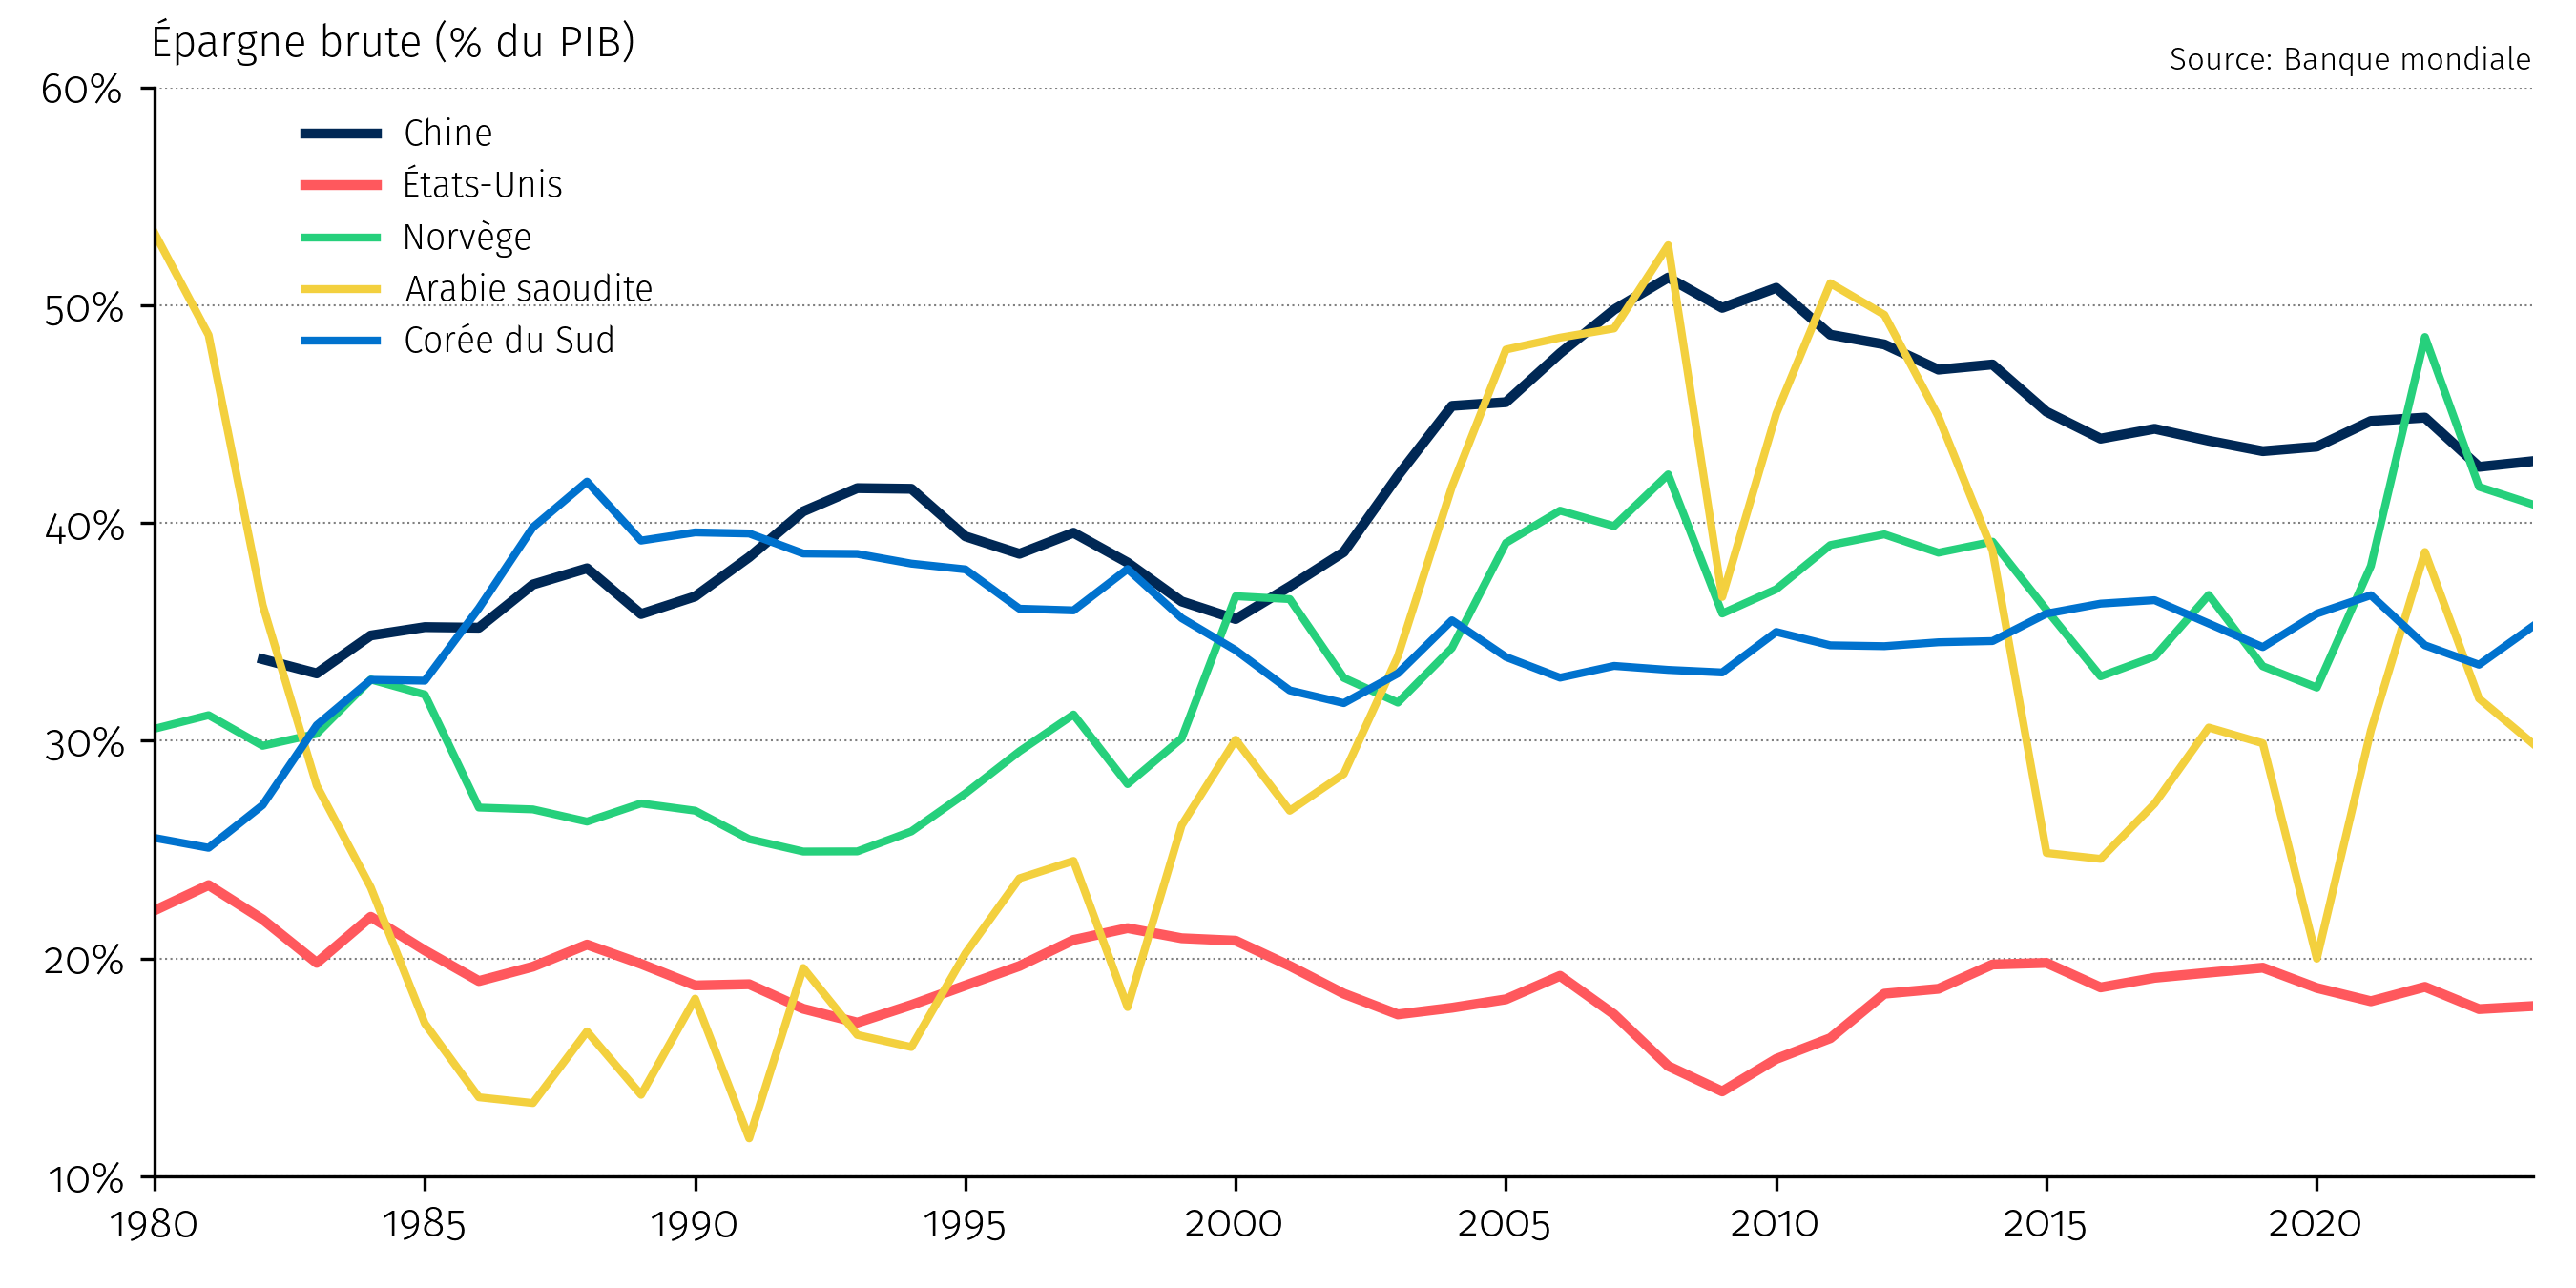
\includegraphics[width=0.95\textwidth, height=0.78\textheight, keepaspectratio]{saving_rates_divergence.png}
   \end{figure}
\end{frame}

\begin{frame}[t]{Hypothèse 3 --- le diagramme}
   \centering
   \vfill
   % S^w shifts RIGHT by 1.6 in q (saving glut from ROW)
   %   New S^w': r = 0.42q - 0.54
   %   New eq: q = 4.64, r = 1.41
   % At r^w' = 1.41: S_H = 1.88, I_H = 4.12, CA = -2.24
   \begin{tikzpicture}[scale=0.9]
      % ── Panel 1: World ──────────────────────────
      \begin{scope}[xshift=0cm]
         \node[font=\normalsize\bfseries, text=HECnavy] at (3.25,5.2) {Monde};
         % Old r^w (faded)
         \draw[HECgreen!40, thick, dotted] (0,1.8) -- (6.5,1.8);
         \node[left, pointlabel, text=HECgray] at (0,1.8) {$r^w$};
         % New r^w' (green dotted)
         \draw[HECgreen, very thick, dotted] (0,1.41) -- (6.5,1.41);
         % I^w unchanged
         \draw[very thick, HECcoral] (0,4.42) -- (6.0,0.52)
            node[above, xshift=-2pt, curvelabel, text=HECcoral] {$I^w$};
         % Original S^w (dashed gray)
         \draw[original] (0,0.13) -- (6.0,2.65)
            node[above, xshift=-4pt, font=\small, text=HECgray] {$S^w$};
         % New S^w' (shifted right): r = 0.42q - 0.54
         \draw[curveshift, HECgreen] (1.29,0) -- (6.2,2.06)
            node[above left, curvelabel, text=HECgreen] {$S^{w\prime}$};
         % Shift arrow
         \draw[shiftarrow, HECgreen] (4.0,1.55) -- (5.0,1.55);
         \node[font=\scriptsize, HECgreen, above] at (4.5,1.55) {$S^w_R \uparrow$};
         % Old equilibrium (faded)
         \filldraw[eqfaded] (4.01,1.8) circle (2.5pt);
         % New equilibrium
         \draw[refline, HECgreen] (4.64,0) node[below, pointlabel, text=HECgreen] {$S^{w\prime} = I^w$} -- (4.64,1.41);
         \node[left, pointlabel, text=HECgreen] at (0,1.41) {$r^{w\prime}$};
         \filldraw[eqpoint=HECgreen] (4.64,1.41) circle (3pt);
         % Axes
         \draw[econaxis] (0,0) -- (6.5,0) node[right] {$S, I$};
         \draw[econaxis] (0,0) -- (0,4.8) node[above] {$r$};
      \end{scope}

      % ── Panel 2: É.-U. ────────────────────────
      \begin{scope}[xshift=7.5cm]
         \node[font=\normalsize\bfseries, text=HECnavy] at (3.0,5.2) {É.-U.};
         % Old r^w (faded)
         \draw[HECgreen!40, thick, dotted] (0,1.8) -- (5.8,1.8);
         \node[left, pointlabel, text=HECgray] at (0,1.8) {$r^w$};
         % New r^w' (green dotted)
         \draw[HECgreen, very thick, dotted] (0,1.41) -- (5.8,1.41);
         \node[left, pointlabel, text=HECgreen] at (0,1.41) {$r^{w\prime}$};
         % Shift arrow on r^w
         \draw[shiftarrow, HECgreen] (-0.15,1.72) -- (-0.15,1.49);
         % S_H unchanged
         \draw[very thick, HECnavy] (0,0) -- (5.5,4.125)
            node[above left, curvelabel, text=HECnavy] {$S_H$};
         % I_H unchanged
         \draw[very thick, HECcoral] (0,4.5) -- (6.0,0)
            node[above, curvelabel, text=HECcoral] {$I_H$};
         % Old allocations (faded)
         \filldraw[eqfaded] (2.4,1.8) circle (2pt);
         \filldraw[eqfaded] (3.6,1.8) circle (2pt);
         % New allocations at r^w' = 1.41
         \draw[refline] (1.88,0) node[below, pointlabel] {$S_H'$} -- (1.88,1.41);
         \draw[refline] (4.12,0) node[below, pointlabel] {$I_H'$} -- (4.12,1.41);
         \filldraw[eqpoint=HECnavy] (1.88,1.41) circle (2.7pt);
         \filldraw[eqpoint=HECcoral] (4.12,1.41) circle (2.7pt);
         % CA deficit brace
         \draw[decorate, decoration={brace, amplitude=8pt, mirror}, very thick, HECcoral]
            (1.88,-0.55) -- (4.12,-0.55)
            node[midway, below=8pt, font=\small\bfseries, text=HECcoral] {$CA \downarrow\downarrow$};
         % Axes
         \draw[econaxis] (0,0) -- (6.2,0) node[right] {$S, I$};
         \draw[econaxis] (0,0) -- (0,4.8) node[above] {$r$};
      \end{scope}
   \end{tikzpicture}
   \vfill
   \centering
   {\small Prédiction : $CA \downarrow$ \textcolor{HECgreen}{\checkmark} \quad et \quad $r^w \downarrow$ \textcolor{HECgreen}{\checkmark} \quad --- \textbf{correspond aux données\,!}}
\end{frame}

\begin{frame}[t]{Bilan : l'excès d'épargne résout le puzzle}
   \small
   \vspace{0.1cm}
   \renewcommand{\arraystretch}{1.5}
   \centering
   \begin{tabularx}{0.9\textwidth}{>{\small}X >{\small\centering}p{2.5cm} >{\small\centering\arraybackslash}p{2.5cm}}
      \toprule
      & \textbf{$CA$} & \textbf{$r^w$} \\
      \midrule
      \textbf{Données observées} & $\downarrow$ & $\downarrow$ \\
      \midrule
      $S_G \downarrow$ (déficits budg.) & $\downarrow$ \textcolor{HECgreen}{\checkmark} & $\uparrow$ \textcolor{HECcoral}{$\boldsymbol{\times}$} \\
      $I_H \uparrow$ (boom techno) & $\downarrow$ \textcolor{HECgreen}{\checkmark} & $\uparrow$ \textcolor{HECcoral}{$\boldsymbol{\times}$} \\
      \rowcolor{HECgreen!10}
      $S^w_R \uparrow$ (épargne mondiale) & $\downarrow$ \textcolor{HECgreen}{\checkmark} & $\downarrow$ \textcolor{HECgreen}{\checkmark} \\
      \bottomrule
   \end{tabularx}
   \vspace{0.3cm}
   \begin{bizimplication}
      \footnotesize
      Les déséquilibres mondiaux ne sont pas le résultat de \guillemotleft~mauvais comportements~\guillemotright\ d'un seul pays. Ils reflètent des forces macroéconomiques profondes (démographie, développement financier, politique industrielle) dans \textbf{plusieurs} pays simultanément.
   \end{bizimplication}
\end{frame}

% ============================================================================

\begin{frame}{Plan}
   \begin{enumerate}
      \setlength\itemsep{0.4cm}
      \item {\color{gray!50}La mondialisation en question}
      \item {\color{gray!50}D'où viennent les déficits commerciaux\,?}
      \item {\color{gray!50}Le modèle épargne-investissement}
      \item {\color{gray!50}Le puzzle américain et l'excès d'épargne mondiale}
      \item \textbf{Les tarifs corrigent-ils le déficit\,?}
      \item Géoéconomie : au-delà du modèle standard
      \item Récapitulatif du cours
   \end{enumerate}
\end{frame}

% ============================================================================
\sectionframe{Les tarifs corrigent-ils le déficit\,?}
% ============================================================================

\begin{frame}[t]{Les tarifs dans l'actualité}
   \small
   \vspace{0.2cm}
   Nous avons maintenant les outils pour répondre à notre \textbf{troisième question} : les tarifs peuvent-ils corriger le déficit commercial\,?
   \vspace{0.2cm}

   En séance 4, nous avons vu l'effet des tarifs comme \textbf{choc d'offre} dans le modèle AD-AS.
   \vspace{0.15cm}
   \begin{itemize}
      \setlength\itemsep{0.2cm}
      \item Les tarifs augmentent les coûts de production $\to$ AS se déplace vers la gauche
      \item Résultat : $Y \downarrow$ et $P \uparrow$ (stagflation)
   \end{itemize}
   \vspace{0.2cm}
   Maintenant, analysons leur effet sur la \textbf{balance commerciale} avec le modèle S-I.

   \vspace{0.2cm}
   {\large La question centrale : les droits de douane peuvent-ils réduire le déficit commercial\,?}
\end{frame}

\begin{frame}[t]{Les tarifs et le modèle S-I}
   \small
   \vspace{0.1cm}
   \begin{warning}[Le point analytique clé]
      \footnotesize
      Puisque $CA = S - I$, les droits de douane ne peuvent réduire le déficit commercial \textbf{que s'ils modifient $S$ ou $I$}.
   \end{warning}
   \vspace{0.15cm}
   \begin{columns}[T]
      \begin{column}{0.47\textwidth}
         \textbf{Que font les tarifs au marché des biens\,?}
         \begin{itemize}
            \setlength\itemsep{0.1cm}
            \item Réduisent les importations de certains pays
            \item Augmentent les prix domestiques
            \item Provoquent des représailles
         \end{itemize}
      \end{column}
      \begin{column}{0.47\textwidth}
         \textbf{Mais que font-ils à $S$ et $I$\,?}
         \begin{itemize}
            \setlength\itemsep{0.1cm}
            \item Ne changent pas l'épargne nationale
            \item Ne changent pas l'investissement
            \item Donc $CA = S - I$ est \textbf{inchangé}
         \end{itemize}
      \end{column}
   \end{columns}
\end{frame}

\begin{frame}[t]{L'évidence empirique}
   \small
   \vspace{0.1cm}
   \textbf{Les tarifs de 2018 sur la Chine :}
   \vspace{0.15cm}
   \begin{itemize}
      \setlength\itemsep{0.2cm}
      \item Le déficit commercial des É.-U.\ \textbf{avec la Chine} a diminué
      \item Mais le déficit commercial \textbf{total} des É.-U.\ est resté essentiellement inchangé
      \item Les importations se sont simplement \textbf{redirigées} : du Vietnam, du Mexique, de l'ASEAN
   \end{itemize}
   \vspace{0.15cm}
   % TODO: Replace placeholder with actual figure (Census Bureau data)
   \begin{tcolorbox}[colback=HEClightgray, colframe=HECgray, boxrule=0.5pt, arc=8pt,
      width=0.9\textwidth, height=3cm, valign=center]
      \centering
      \textcolor{HECgray}{\small [Figure : Déficit commercial É.-U.\ : total vs avec la Chine (2017--2025)]}\\
      \textcolor{HECgray}{\small Source : U.S.\ Census Bureau}
   \end{tcolorbox}
\end{frame}

\begin{frame}[t]{Le grand enseignement}
   \begin{keyinsight}[Le message central]
      Les droits de douane ne corrigent pas les déficits commerciaux --- ils ne font que \textbf{rediriger} les flux commerciaux. Pour réduire le déficit, il faudrait augmenter l'épargne ou réduire l'investissement.
   \end{keyinsight}
   \vspace{0.1cm}
   \begin{bizimplication}
      Pour les entreprises, les tarifs créent de l'incertitude et des réorganisations coûteuses des chaînes d'approvisionnement, sans résoudre le problème sous-jacent.
   \end{bizimplication}
   \mbox{}\hfill{\scriptsize\textcolor{HECgray}{La vraie question : \guillemotleft~pourquoi l'Amérique épargne-t-elle si peu\,?~\guillemotright}}
\end{frame}

% ============================================================================

\begin{frame}{Plan}
   \begin{enumerate}
      \setlength\itemsep{0.4cm}
      \item {\color{gray!50}La mondialisation en question}
      \item {\color{gray!50}D'où viennent les déficits commerciaux\,?}
      \item {\color{gray!50}Le modèle épargne-investissement}
      \item {\color{gray!50}Le puzzle américain et l'excès d'épargne mondiale}
      \item {\color{gray!50}Les tarifs corrigent-ils le déficit\,?}
      \item \textbf{Géoéconomie : au-delà du modèle standard}
      \item Récapitulatif du cours
   \end{enumerate}
\end{frame}

% ============================================================================
\sectionframe{Géoéconomie : au-delà du modèle standard}
% ============================================================================

% TODO: Populate this section. Possible topics:
% - Weaponization of interdependence (Farrell & Newman)
% - Sanctions as economic statecraft (Russia, Iran)
% - Friend-shoring and supply chain security
% - Dollar dominance and the SWIFT system
% - Rare earth dependencies and industrial policy
% - Digital trade barriers and data sovereignty

\begin{frame}[t]{Au-delà de l'avantage comparatif}
   \vspace{0.2cm}
   Le modèle S-I explique les \textbf{flux} commerciaux, mais pas les \textbf{rapports de force}.
   \vspace{0.2cm}
   \begin{itemize}
      \setlength\itemsep{0.25cm}
      \item Pourquoi les É.-U.\ utilisent-ils le dollar comme \textbf{arme}\,?
      \item Pourquoi la Chine contrôle-t-elle 60\,\% des terres rares\,?
      \item Pourquoi les sanctions contre la Russie n'ont-elles que partiellement fonctionné\,?
      \item Comment le Canada doit-il naviguer entre ses deux partenaires\,?
   \end{itemize}
   \vspace{0.2cm}
   \begin{keyinsight}
      Le commerce international n'est pas seulement une question d'efficacité économique --- c'est aussi une question de \textbf{pouvoir}.
   \end{keyinsight}
\end{frame}

% ============================================================================

\begin{frame}{Plan}
   \begin{enumerate}
      \setlength\itemsep{0.4cm}
      \item {\color{gray!50}La mondialisation en question}
      \item {\color{gray!50}D'où viennent les déficits commerciaux\,?}
      \item {\color{gray!50}Le modèle épargne-investissement}
      \item {\color{gray!50}Le puzzle américain et l'excès d'épargne mondiale}
      \item {\color{gray!50}Les tarifs corrigent-ils le déficit\,?}
      \item {\color{gray!50}Géoéconomie : au-delà du modèle standard}
      \item \textbf{Récapitulatif du cours}
   \end{enumerate}
\end{frame}

% ============================================================================
\sectionframe{Récapitulatif du cours}
% ============================================================================

\begin{frame}[t]{Le fil conducteur}
   \small
   \vfill
   \renewcommand{\arraystretch}{1.5}
   \centering
   \begin{tabularx}{\textwidth}{>{\bfseries\small}c >{\small}X >{\small\raggedright\arraybackslash}X}
      \toprule
      & \textbf{Thème} & \textbf{Question centrale} \\
      \midrule
      S1 & PIB, inflation, niveau de vie & Comment mesurer l'économie\,? \\
      S2 & Croissance de long terme & Pourquoi certains pays sont riches\,? \\
      S3 & Marché du travail, inégalités, IA & Qui profite de la croissance\,? \\
      S4 & Cycles économiques & Pourquoi l'économie fluctue\,? \\
      S5 & Politique monétaire et budgétaire & Comment stabiliser l'économie\,? \\
      S6 & Commerce international & L'économie dans un monde ouvert \\
      \bottomrule
   \end{tabularx}
   \vfill
\end{frame}

\begin{frame}[t]{Ce que vous devriez retenir}
   \small
   \vspace{0.1cm}
   \begin{enumerate}
      \setlength\itemsep{0.3cm}
      \item \textbf{La macro, c'est concret} --- chaque concept se traduit en décisions d'affaires
      \item \textbf{Les identités comptables disciplinent la réflexion} --- $Y = C + I + G + NX$ et $CA = S - I$ sont des garde-fous contre les raisonnements fallacieux
      \item \textbf{Le long terme et le court terme sont différents} --- ce qui est bon pour la croissance (épargne, investissement) n'est pas toujours bon pour la stabilisation
      \item \textbf{Les politiques ont des effets secondaires} --- les tarifs ne corrigent pas les déficits, la relance budgétaire augmente la dette, la politique monétaire agit avec retard
      \item \textbf{Tout est interconnecté} --- dans un monde ouvert, les décisions d'un pays affectent tous les autres
   \end{enumerate}
\end{frame}

% ============================================================================
% CLOSING SEQUENCE
% ============================================================================

\begin{frame}{}
   \centering
   \vspace{1.5cm}
   {\Large\textbf{Qu'est-ce que vous retenez de ce cours\,?}}
\end{frame}

\end{document}
